\documentclass[a4paper,12pt,oneside]{book}
\usepackage[T1]{fontenc}
%\usepackage[utf8]{inputenc}
\usepackage[italian]{babel}
\usepackage{hyperref}
\usepackage{graphicx}
\usepackage{wrapfig}
\usepackage{makeidx}
\usepackage[table]{}
\usepackage{ragged2e}
\usepackage{multirow}
\usepackage{caption}
\usepackage{floatrow}
\usepackage{amssymb}
\usepackage{amsmath}
\usepackage{tikz}
\usepackage[ruled,vlined]{algorithm2e}
\usepackage[paper=a4paper,margin=1in]{geometry}

\geometry{margin=1.8cm}

\graphicspath{{./images/}}

\begin{document}

\frontmatter
    \title{Allineamento Wavefront per l'individuazione di ricombinazioni}
\author{Volpato Mattia}
\date{21/07/2023}

\pagenumbering{gobble} % Per evitare il page numbering, usate il package che preferite e poi togliete questa linea
\setlength\intextsep{0pt}
\begin{wrapfigure}[4]{l}{5\baselineskip}
    \vspace{-0.25\baselineskip}
    
\includegraphics[width=5\baselineskip]{images/logo_bicocca.png}
\end{wrapfigure}
\noindent
Università degli Studi di Milano Bicocca \\[8pt]
\textbf{Scuola di Scienze} \\[8pt]
\textbf{Dipartimento di Informatica, Sistemistica e Comunicazione}\\[8pt]
\textbf{Corso di laurea in Informatica}

\vspace{30mm}

\begin{center}
    \Huge
    \textbf{Allineamento wavefront per l'individuazione di ricombinazioni}
\end{center}

\vspace{60mm}

\large
\noindent
\textbf{Relatore:} Gianluca Della Vedova \\[7pt]
\textbf{Co-relatore:} Paola Bonizzoni \\[20pt]
\begin{flushright}
\textbf{Relazione della prova finale di:} \\[7pt]
Volpato Mattia \\[7pt]
Matricola 866316
\end{flushright}
\vspace{30mm}
\centering
\textbf{Anno Accademico 2022-2023}
    \justifying
    \chapter{Abstract}
L'\textbf{allineamento di sequenze genomiche} è una parte fondamentale della biologia molecolare moderna, che permette di individuare regioni di somiglianza all'interno delle sequenze nucleotidiche. I progressi degli ultimi anni nelle tecnologie di sequenziamento hanno permesso di avere a disposizione sequenze di lunghezza sempre maggiore, oltre a una quantità notevole di dati; per riuscire a sfruttare a pieno questi progressi tecnologici è necessario riuscire a sviluppare algoritmi di allineamento più veloci ed efficienti, che riescano a scalare con la crescita delle sequenze da allineare. In questo lavoro viene presentato l'\textbf{algoritmo \textit{wavefront}}, un nuovo approccio di programmazione dinamica per l'allineamento di sequenze basato sull'astrazione del \emph{fronte d'onda}: nella prima parte viene riportata la letteratura sul tema dell'allineamento, partendo da coppie di sequenze e successivamente generalizzando a strutture a grafo; nella seconda parte viene presentato l'algoritmo \textbf{\textit{wavefront}}, partendo sempre dal caso più semplice di due sequenze per poi passare a estensioni sui grafi; infine, nella terza parte viene presentato un prototipo realizzato per l'implementazione dell'algoritmo, procedendo con un confronto con \emph{Recgraph}, un tool sviluppato in precedenza dal laboratorio \href{https://algolab.eu/}{BIAS} che effettua allineamento con metodologie standard.

\tableofcontents
    
\mainmatter
    \chapter{Introduzione}
\section{La bioinformatica}
    La \textbf{bioinformatica} è una disciplina che combina la \textbf{biologia}, l'\textbf{informatica} e la \textbf{statistica} per analizzare, elaborare e interpretare i dati biologici utilizzando \emph{strumenti computazionali}. Con l'avvento delle tecnologie di sequenziamento di \emph{DNA} e \emph{RNA} ad alta velocità il volume di dati biologici generati è aumentato a dismisura, rendendo necessario integrare un approccio computazionale nelle metodologie di analisi biologica. La bioinformatica risulta quindi indispensabile per gestire, analizzare e trarre informazioni significative dall'enorme quantità di dati che viene generata.
    
    Questa disciplina di recente nascita svolge un ruolo fondamentale in molteplici ambiti della biologia, trovando un'applicazione a diverse componenti della letteratura informatica sviluppata negli anni passati. Attraverso l'uso di algoritmi, modelli statistici e metodi computazionali, la \textbf{bioinformatica} consente, tra le altre cose, di analizzare sequenze genetiche, identificare geni, annotare genomi, studiare l'evoluzione e predire la struttura delle proteine.
    
    In particolare, una componente che si dimostra cruciale in queste specifiche applicazioni è l'\textbf{allineamento di sequenze}, risultando uno strumento fondamentale per analizzare le similarità e le differenze tra le sequenze biologiche.

\section{Applicazioni dell'allineamento di sequenze}
    Uno dei principi ampiamenti riconosciuti nella \textbf{biologia molecolare}, che si pone come uno dei pilastri di questa disciplina, è il seguente:
    \begin{quote}
         Nelle \textbf{sequenze biomolecolari} (\emph{DNA, RNA o sequenze amminoacide}), \textbf{un'alta similarità delle sequenze} di solito implica \textbf{significative similarità funzionali e/o strutturali}. \cite{Gusfield}
    \end{quote}
    Il fatto che due sequenze biomolecolari presentino un'alta similarità significa che esse condividono una notevole quantità di informazioni genetiche o strutturali. Questo può indicare che le due sequenze derivino da organismi strettamente correlati o che svolgano funzioni simili.

    In particolare, la \textbf{similarità funzionale} può indicare che le sequenze condividono una specifica attività biologica o svolgono un ruolo simile all'interno di un processo biologico, mentre la \textbf{similarità strutturale} si riferisce alla conservazione della struttura tridimensionale delle biomolecole: sequenze con alta similarità strutturale possono indicare comformazioni simili per le proteine corrispondenti. Tuttavia, è importante notare che non sempre la similarità delle sequenze garantisce una funzionalità o struttura identica: esistono infatti diversi casi in cui questo non accade. 
    
    Di conseguenza, l'allineamento di sequenze risulta fondamentale nella ricerca di \textbf{regioni conservate}, che sono segmenti di sequenze simili o addirittura identiche: esse spesso indicano l'esistenza di una funzione biologica comune o di una relazione evolutiva condivisa. Un esempio sono le sequenze proteiche, in cui regioni conservate possono rivelare la presenza di motivi strutturali o di siti attivi importanti per la loro funzione.
    
    Un'altra applicazione importante dell'allineamento è l'\textbf{identificazione di variazioni o mutazioni}. Durante l'evoluzione, le sequenze nucleotidiche subiscono cambiamenti a livello genetico (ad esempio \emph{mutazioni puntiformi}, \emph{inserzioni} o \emph{delezioni}). L'allineamento mette in evidenza le differenze tra le sequenze, permettendo di individuare queste mutazioni e di studiare il loro impatto sulla struttura e sulla funzione delle biomolecole. Un esempio di questa applicazione è il campo della ricerca sulle malattie genetiche, dove l'allineamento di sequenze genomiche può rivelare varianti genetiche associate a condizioni patologiche.
    
    Inoltre, i risultati forniti dall'allineamento vengono utilizzati anche all'interno di altri campi della bioinformatica: nella costruzione degli \textbf{alberi filogenetici}, utilizzati per rappresentare storie e relazioni evolutive, vengono usati gli allineamenti di sequenze nucleotidiche per stimare la \emph{distanza evolutiva} di specie diverse.

\section{Tecnologie di sequenziamento}
    Uno dei principali motivi dei progressi nei campi della biologia e della genetica sono le \textbf{tecnologie di sequenziamento}, un insieme di metodi e strumenti utilizzati per determinare l'ordine esatto dei nucleotidi (A, C, G, T) all'interno di una molecola di \emph{DNA} o \emph{RNA}. Il loro sviluppo ha consentito la generazione di quantità sempre crescenti e di maggior qualità di dati genomici, in modo rapido ed efficiente.

\clearpage

\begin{figure}[ht]
%\hspace*{-2cm}
\centering
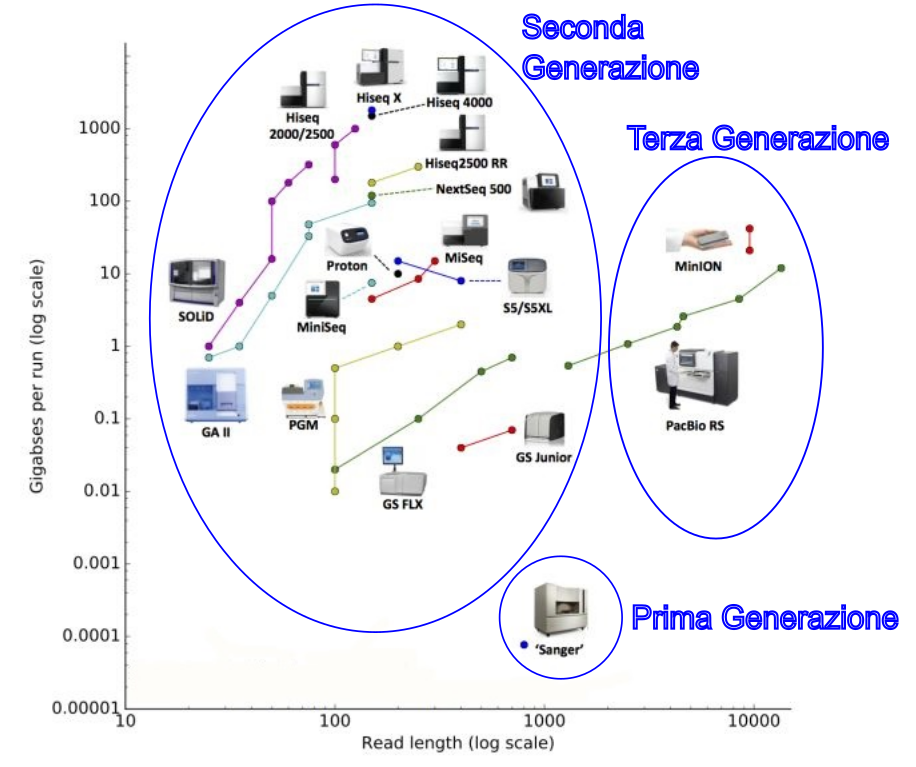
\includegraphics[width=1\linewidth]{images/sequencing_technologies.png} 
\caption[Tecnologie di sequenziamento]{Suddivisione delle \emph{tecnologie di sequenziamento} in generazioni.}
\label{fig:tecnologie_sequenziamento}
\end{figure}
\vspace{30pt}
\noindent
Come si vede dalla figura \ref{fig:tecnologie_sequenziamento}, è possibile dividere le \textbf{tecnologie di sequenziamento} in \textbf{tre generazioni}:
\begin{itemize}
    \item \textbf{Prima generazione}:
    tecnologie conosciute anche come \emph{sequenziamento  Sanger}, sono state usate nel progetto \emph{Genoma Umano} per riuscire a ricostruire l'intero patrimonio genetico di un essere umano; producono sequenze di \emph{lunghezza} pari a circa 1000 nucleotidi con un \emph{throughput}\footnote{Per \emph{throughput} si intende la quantità di dati prodotta in un determinato lasso di tempo (nella figura \ref{fig:tecnologie_sequenziamento} Gigabasi per esecuzione).} limitato, insieme a un \emph{tasso di errore} del $6\%$ circa;

    \item \textbf{Seconda generazione}:
    la classe di tecnologie più sviluppata, hanno come punto di forza un \emph{elevato throughput}, mantenendo anche un \emph{basso tasso di errore} ($<1\%$) e \emph{lunghezza delle sequenze} abbastanza variabile, sempre però al di sotto delle 1000 bp\footnote{bp sta per \emph{base pair}, che indica una coppia di nucleotidi; viene usata come unità di misura per la lunghezza delle sequenze generitiche.} del \emph{sequenziatore Sanger}; hanno però il limite di produrre \emph{errori sistematici} sempre dello stesso tipo; 

    \item \textbf{Terza generazione}:
    classe ancora in forte sviluppo, si concentrano sulla produzione di sequenze di \emph{elevata lunghezza} (quasi 10000 nucleotidi per sequenza), mantenendo un \emph{throughput} abbastanza elevato. Producono \emph{errori} con un tasso piuttosto elevato (più del $10\%$), che sono però distribuiti in maniera \emph{casuale}. 
\end{itemize}
La tabella \ref{tab:errori_sequenziatori} riporta in maniera strutturata le caratteristiche delle varie generazioni di \emph{tecnologie di sequenziamento}.

\vspace{30pt}
\begin{table}[h]
    \centering
    \begin{tabular}{|c|c|c|c|c|}
        \hline
            \multicolumn{5}{|c|}{\textbf{Tecnologie di sequenziamento}} \\
        \hline
            \textbf{Generazione} & \textbf{Sequenze} & \textbf{Throughput} & \textbf{Tasso di errore} & \textbf{Tipo di errore} \\
        \hline
            Prima & $\approx 1000$ & $< 0.01$ & $\approx 6\%$ & Casuale \\
        \hline
            Seconda & tra 50 e 1000 & fino a $18000$ & $<1\%$ & Sistematico \\
        \hline
            Terza & $\approx 10000$ & $\approx 10$ & $>10\%$ & Casuale \\
        \hline
    \end{tabular}
    \caption{Caratteristiche delle varie generazioni di tecnologie di sequenziamento; il \emph{throughput} è misurato in \emph{Gb/day} e la \emph{lunghezza} delle sequenze in \emph{bp}.}
    \label{tab:errori_sequenziatori}
\end{table}

\section{Obiettivo dello stage}
    L'obiettivo dello stage era quello di effettuare uno studio approfondito dell'algortimo \textbf{\textit{wavefront}}, un nuovo approccio basato sulla \emph{programmazione dinamica} che permette di calcolare la \textbf{distanza di edit} in tempo proporzionale al valore della distanza stessa (capitolo \ref{section:wfa}). 
    
    In particolare, l'obiettivo finale era quello di integrare l'approccio \textbf{\textbf{wavefront}} all'interno di \href{https://github.com/AlgoLab/RecGraph}{\textbf{\textit{RecGraph}}} \cite{Recgraph}, un tool precedentemente sviluppato che permette di effettuare numerosi tipi di allineamenti tra un \emph{grafo} e una \emph{sequenza}, in particolare un allineamento che permette di individuare fino a una \emph{ricombinazione} all'interno del genoma rappresentato nel grafo. 
    
    Nella prima parte del percorso ci si è concentrati sullo studio dell'algoritmo, partendo da una sua applicazione su due sequenze per poi cercare di generalizzarlo su strutture dati più complesse (\textbf{grafi di sequenza} e \textbf{grafi di variazione}).
    
    In una seconda parte si è passati all'implementazione di un prototipo (nel linguaggio \href{https://www.rust-lang.org/it}{\textbf{\textit{Rust}}}) che utilizzasse l'algoritmo \textbf{\textit{wavefront}} per effettuare un allineamento tra \textbf{grafi di variazione} e \textbf{sequenze} e che permettesse di migliorare le capacità computazionali di \textbf{\textit{RecGraph}}, rendendo possibile l'utilizzo di istanze di grafi di dimensioni sempre maggiori.  
    \chapter{Allineamento di sequenze}
    Dopo aver esposto alcuni dei principali motivi per cui l'allineamento di sequenze risulta fondamentale nella \emph{bioinformatica}, si procede con una trattazione formale dell'argomento, partendo dal caso più semplice dell' \textbf{allineamento} di \textbf{due sequenze} fino ad arrivare a una sua generalizzazione tra un \textbf{grafo} e una \textbf{sequenza}. 
    
\section{Allineamento tra due sequenze}
    \textbf{Definizione}: Un \emph{allineamento} di due stringhe $S_1$ e $S_2$ si ottiene inserendo inizialmente gli \emph{spazi} (o \emph{indel}) all'inizio, all'interno o alla fine di $S_1$ e $S_2$, e successivamente allineando le due stringhe una sopra l'altra in maniera tale che, in entrambe le stringhe, ogni carattere o spazio risulti allineato a un singolo carattere o spazio dell'altra sequenza. Due spazi non possono risultare allineati tra loro. \cite{Gusfield}

    Un esempio di un allineamento delle due sequenze $S_1 = abbdcd$ e $S_2 = tbbqddc$ è il seguente:
    \vspace{20pt}
    \begin{table}[h]
        \centering
        \begin{tabular}{ccccccccc}
             a & - & b & b & - & d & c & d \\
             t & b & b & q & d & d & c & - \\
        \end{tabular}
    \end{table}
    \vspace{20pt}

    Una delle possibili metologie per approcciarsi al problema dell'allineamento è la \emph{programmazione dinamica}: infatti esso può essere visto come un \emph{problema di ottimizzazione}, descritto formalmente come segue:  
    
    \noindent
    \textbf{\textit{Input:}} 
    \begin{itemize}
        \item \textbf{Alfabeto} $\Sigma$
        \item \textbf{Sequenza} $X = <x_1, x_2, ..., x_n>, \, x_i \in \Sigma \quad \forall i \in \{1, ..., n\}$
        \item \textbf{Sequenza} $Y = <y_1, y_2, ..., y_m>, \, y_j \in \Sigma \quad \forall j \in \{1, ..., m\}$
        \item \textbf{Matrice di score} $d: (\Sigma \cup \{-\}) \times (\Sigma \cup \{-\}) \rightarrow \mathbb{Q}$
    \end{itemize}
    \textbf{\textit{Output:}} 
    \begin{itemize}
        \item \textbf{Valore dell'allineamento} $s = \sum_{i=1}^{k} d(x_i, y_i)$
    \end{itemize}

    In particolare, \emph{l'insieme delle soluzioni ammissibili} è composto da tutti i possibili allineamenti di $X$ e $Y$ (con eventualmente spazi inseriti all'inizio, all'interno o alla fine delle due stringhe); la \emph{soluzione ottimale} è quella che \emph{massimizza} il punteggio dell'allineamento (\textbf{massima omologia}).
    
\subsection{Equazioni di ricorrenza}
\label{section:needleman-wunsch}
\subsubsection{Dimostrazione di correttezza}
    Si considerino i prefissi delle due stringhe $X$ e $Y$
    \begin{itemize}
        \item $X_i = <x_1, x_2, ..., x_i>$,
        \item $Y_j = <y_1, y_2, ..., y_j>$
    \end{itemize}
    e sia $M[i, j]$ il \emph{valore ottimo} dell'allineamento di $X_{i}$ e $Y_{j}$; è possibile distinguere solo i seguenti casi:
    \begin{itemize}
        \item $x_i$ viene allineato con $y_j$: 
        \vspace{5pt}
        \begin{table}[h]
            \centering
            \begin{tabular}{|cccc|c|}
            \hline
                \multicolumn{4}{|c|}{$X_{i-1}$} & $X_i$\\
            \hline
                $x_0$ & $x_1$ & ... & $x_{i-1}$ & $x_i$ \\
                 $y_0$ & $y_1$ & ... & $y_{j-1}$ & $y_j$ \\
            \hline
                \multicolumn{4}{|c|}{$Y_{j-1}$} & $Y_j$\\
            \hline
            \end{tabular}
        \end{table}
        \vspace{5pt}
        
        in questo caso, il valore ottimo dell'allineamento sarà dato da
        $$M[i, j] = M[i-1, j-1] + d(x_i, y_j)$$
        
        \item $x_i$ viene allineato con '$-$': 
        \vspace{5pt}
        \begin{table}[h]
            \centering
            \begin{tabular}{|cccc|c|}
            \hline
                \multicolumn{4}{|c|}{$X_{i-1}$} & $X_i$\\
            \hline
                $x_0$ & $x_1$ & ... & $x_{i-1}$ & $x_i$ \\
                 $y_0$ & $y_1$ & ... & $y_{j-1}$ & $-$ \\
            \hline
                \multicolumn{4}{|c|}{$Y_{j-1}$} & \\
            \hline
            \end{tabular}
        \end{table}
        \vspace{5pt}
        
        in questo caso, il valore ottimo dell'allineamento sarà dato da
        $$M[i, j] = M[i-1, j] + d(x_i, -)$$
        \clearpage
        
        \item $y_j$ viene allineato con '$-$': 
        \vspace{5pt}
        \begin{table}[h]
            \centering
            \begin{tabular}{|cccc|c|}
            \hline
                \multicolumn{4}{|c|}{$X_{i-1}$} & \\
            \hline
                $x_0$ & $x_1$ & ... & $x_{i-1}$ & $-$ \\
                 $y_0$ & $y_1$ & ... & $y_{j-1}$ & $y_j$ \\
            \hline
                \multicolumn{4}{|c|}{$Y_{j-1}$} & $Y_j$\\
            \hline
            \end{tabular}
        \end{table}
        \vspace{5pt}
        
        in questo caso, il valore ottimo dell'allineamento sarà dato da
        $$M[i, j] = M[i, j-1] + d(-, y_j)$$
    \end{itemize}
    Non si riescono a individuare altre possibilità, quindi i tre casi elencati coprono tutte le casistiche; è possibile scrivere di conseguenza la seguente \emph{equazione di ricorrenza}:
    
    \vspace{20pt}
    \textbf{Needleman-Wunsch} \cite{NeedlemanWunsch}
    \begin{equation}
        M[i, j] = \max \begin{cases}
            M[i-1, j] + d(x_i, -) & \\
            M[i-1, j-1] + d(x_i, y_j) & \\
            M[i, j-1] + d(-, y_j) & \\
        \end{cases}
        \label{needleman-wunsch}
    \end{equation}
    $$\forall i > 0, \, \forall j > 0$$

\subsection{Ricostruzione della soluzione}
\label{subsection:traceback}
    Per ottenere anche l'allineamento effettivo delle due sequenze, è necessario salvare per ogni elemento di $M[i, j]$ la cella da cui è stato computato, in maniera da poter poi ricostruire la soluzione procedendo a ritroso. Formalmente, questo si traduce nel computare un'altra \emph{matrice di programmazione dinamica} di dimensione $(n + 1) \times (m + 1)$ come segue:
   \begin{equation}
        T[i, j] = \begin{cases}
            \uparrow, & se \, \, M[i, j] =  M[i-1, j] + d(x_i, -), \\
            \rotatebox[origin=c]{45}{$\uparrow$}, & se \, \, M[i, j] =  M[i-1, j-1] + d(x_i, y_j), \\
            \leftarrow, & se \, \, M[i, j] =  M[i, j-1] + d(-, y_j), \\
        \end{cases} \quad \forall (i, j) > \underline{0}
        \label{traceback}
    \end{equation}
\centering
    $$
        T[i, 0] = \, \, \uparrow \quad \forall i > 0
    $$
    $$
        T[0, j] = \, \, \leftarrow \quad \forall j > 0
    $$
    
\raggedright
    Una volta trovata la soluzione ottimale, è sufficiente seguire la sequenza delle celle salvate fino a $M[0, 0]$ per ricostruire l'allineamento.

\raggedright
\subsection{Complessità computazionale}
\label{section:needleman-wunsch_complexity}
\subsubsection{Complessità in tempo}
    Per calcolare l'allineamento ottimale, è necessario computare una matrice di dimensione $(n + 1) \times (m + 1)$, dove ogni elemento viene calcolato in $\Theta(1)$ (equazioni \ref{needleman-wunsch} e \ref{traceback}); di conseguenza, la \emph{complessità temporale} dell'algoritmo sarà data da:
    \begin{equation*}
        T(n, m) = \Theta(nm)
    \end{equation*}

    Per ricostruire la soluzione, invece, è necessario ripercorrere a ritroso il percorso ottimale all'interno della matrice; nel caso migliore questo significa muoversi sempre in diagonale fino alla cella iniziale, mentre nel caso peggiore si seguirà un percorso composto unicamente da passi orizzontali e verticali. In ogni caso, la complessità risulta minore della computazione della matrice: nel \textbf{caso migliore} è \emph{limitata inferiormente} da
    \begin{equation*}
        T(n, m) = \Omega(\max\{n, m\})
    \end{equation*}
    mentre nel \textbf{caso peggiore} risulta \emph{limitata superiormente} da
    \begin{equation*}
        T(n, m) = O(n + m)
    \end{equation*}
    
\subsubsection{Complessità in spazio}
    Ogni elemento della matrice occupa una quantità di memoria \emph{costante}, quindi, in maniera analoga, la \emph{complessità spaziale}\footnote{Se si è interessati solo al \emph{valore dell'allineamento} e non alla \emph{ricostruzione della soluzione}, non è necessario salvare tutta la matrice, ma basta mantenere una sola riga (o colonna, a seconda di come la si computa) per volta. La \textbf{complessità spaziale} risulta quindi $\Theta(\min \{n, m \})$.} sarà:
    \begin{equation*}
        M(n, m) = \Theta(nm)
    \end{equation*}

\subsection{Caso globale}
\subsubsection{Condizioni al contorno}
    
    Nel \textbf{caso globale}, l'obiettivo è quello di allineare completamente le due stringhe: come conseguenza, l'allineamento deve inizare dal primo simbolo e finire all'ultimo, per entrambe le sequenze. Formalmente, questo si traduce nelle seguenti \emph{condizioni al contorno}:

    \begin{equation}
        M[i, j] = \begin{cases}
            0 & i = 0, j = 0 \\
            M[i-1, 0] + d(x_i, -) & i > 0, j = 0\\
            M[0, j-1] + d(-, y_j) & i = 0, j > 0\\
        \end{cases}
    \end{equation}

    La \textbf{soluzione ottima} è data dall'allineamento di entrambe le sequenze nella loro interezza: 
    \begin{equation}
        s = M[n, m]
    \end{equation}
    
\subsubsection{Esempio}
    Di seguito un esempio dell'\textbf{allineamento globale} ottimale di due sequenze nucletotidiche:
    
    \vspace{20pt}
    \noindent \textbf{\textit{Input}}
    \begin{itemize}
        \item $\Sigma$ = \{A, G, C, T\} 
        \item $X$ = "GAATTCAGTTA"
        \item $Y$ = "GGATCGA"
        \item $d(x, y) = \begin{cases}
            5 & \forall x, y \in \Sigma \mid x = y, \\
            -3 & \forall x, y \in \Sigma \mid x \neq y, \\
            -4 & \forall x \in \Sigma, y = -, \\
            -4 & x = -, \forall y \in \Sigma
        \end{cases}$
    \end{itemize}
    
    \noindent
    \textbf{\textit{Output}}
    
    \centering \textbf{Score} = 11
    \vspace{20pt}
    \begin{table}[h]
        \centering
        \begin{tabular}{ccccccccccc}
             G & A & A & T & T & C & A & G & T & T & A \\
             | &   & | &   & | & | &   & | &   &   & | \\
             G & G & A & - & T & C & - & G & - & - & A \\
             \hline
             +5 & -3 & +5 & -4 & +5 & +5 & -4 & +5 & -4 & -4 & +5 \\
             \hline
        \end{tabular}
    \end{table}
    \vspace{20pt}

\raggedright
\subsection{Caso semiglobale}
\subsubsection{Condizioni al contorno}

    Nel \textbf{caso semiglobale}, la seconda sequenza (chiamata solitamente \emph{query} o \emph{read}) può essere allineata a una qualsiasi \emph{sottostringa} della prima (chiamata \emph{testo}): in altre parole, è possibile inserire un numero qualsiasi di \emph{spazi} all'inizio e alla fine della \emph{read} senza penalità aggiuntive. Definita quindi $X$ come la \textbf{sequenza di riferimento} e $Y$ come la \textbf{query} da allineare, questo si traduce nelle seguenti \emph{condizioni al contorno}:

    \begin{equation}
        M[i, j] = \begin{cases}
            0 & i \geq 0, j = 0 \\
            M[0, j - 1] + d(-, y_j) & i = 0, j > 0 \\
        \end{cases}
    \end{equation}

    La \textbf{soluzione ottima} sarà data dall'allineamento che comprende tutta la \emph{read} e una qualsiasi sottostringa del \emph{testo} e che \emph{massimizza il punteggio}, ovvero: 
    \begin{equation}
        s = \max_{0 \leq i \leq n} M[i, m]
    \end{equation}
    
\subsubsection{Esempio}
    Di seguito un esempio dell'\textbf{allineamento semiglobale} ottimale di due sequenze nucletotidiche:

    \vspace{20pt}
    \noindent \textbf{\textit{Input}}
    \begin{itemize}
        \item $\Sigma$ = \{A, G, C, T\} 
        \item $X$ = "GAATTCAGTTA"
        \item $Y$ = "AAACGGT"
        \item $d(x, y) = \begin{cases}
            5 & \forall x, y \in \Sigma \mid x = y, \\
            -3 & \forall x, y \in \Sigma \mid x \neq y, \\
            -4 & \forall x \in \Sigma, y = -, \\
            -4 & x = -, \forall y \in \Sigma
        \end{cases}$
    \end{itemize}

    \noindent \textbf{\textit{Output}}
    
\centering 
    \textbf{Score} = 23
    \vspace{20pt}
    \begin{table}[h]
        \centering
        \begin{tabular}{ccccccccccc}
             G & A & A & T & T & C & G & G & T & T & A \\
               & | & | &   &   & | & | & | & | &   &  \\
             - & A & A & - & A & C & G & G & T & - & - \\
             \hline
             0 & +5 & +5 & -4 & -3 & +5 & +5 & +5 & +5 & 0 & 0 \\
             \hline
        \end{tabular}
    \end{table}
    \vspace{20pt}

\raggedright
\section{Distanza di edit tra due sequenze}
\label{section:edit-distance}
    Un'altra possibilità per misurare quanto due sequenze sono simili tra loro è calcolare la \textbf{distanza} che le divide; in particolare, ci sono numerose maniere con cui viene formalizzata la \emph{distanza tra due stringhe}: una delle più utilizzate è la \textbf{\textit{distanza di edit}}, la quale fornisce il minimo numero di operazioni necessarie a trasformare una stringa nell'altra (oltre all'effettiva sequenza di operazioni necessarie).
    \vspace{20pt}
    
    \textbf{Definizione}: La \emph{distanza di edit} tra due sequenze è definita come il \emph{minimo} numero di \emph{operazioni di edit} - \textbf{inserimenti, cancellazioni e sostituzioni} - necessarie a trasformare la prima sequenza nella seconda. \cite{Gusfield}
    \vspace{20pt}
    
    Si noti che la \textbf{distanza di edit} riferita alla trasformazione della prima sequenza nella seconda è sempre uguale a quella che si riferisce alla trasformazione opposta: è inoltre possibile passare da un \textbf{edit transcript} al duale semplicemente invertendo le operazioni effettuate.

    In maniera analoga all'\textbf{allineamento di sequenze}, anche il problema della \textbf{distanza di edit} può essere risolto in maniera efficiente tramite \emph{programmazione dinamica}:
    \vspace{20pt}
    
    \noindent \textbf{\textit{Input:}} 
    \begin{itemize}
        \item \textbf{Alfabeto} $\Sigma$
        \item \textbf{Sequenza} $X = <x_1, x_2, ..., x_n>, \, x_i \in \Sigma \quad \forall i \in \{1, ..., n\}$
        \item \textbf{Sequenza} $Y = <y_1, y_2, ..., y_m>, \, y_j \in \Sigma \quad \forall j \in \{1, ..., m\}$
    \end{itemize}
    \textbf{\textit{Output:}} 
    \begin{itemize}
        \item \textbf{Distanza di edit} $d$
        \item \textbf{Sequenza} delle \textbf{operazioni di edit} (\textbf{edit transcript})
    \end{itemize}

    \emph{L'insieme delle soluzioni ammissibili} è composto da tutte gli \textbf{edit transcript} che trasformano $X$ in $Y$; la \emph{soluzione ottimale} è quella che minimizza il numero delle \emph{operazioni di edit}.
    
\subsection{Equazioni di ricorrenza}
\subsubsection{Dimostrazione di correttezza}
    Si considerino i prefissi delle due stringhe $X_i = <x_1, x_2, ..., x_i>$, $Y_j = <y_1, y_2, ..., y_j>$ e siano noti
    \begin{itemize}
        \item $D[i, j]$, il \emph{valore ottimo} della distanza di edit tra $X_{i}$ e $Y_{j}$;
        \item $S[i, j]$, l'insieme delle \emph{operazioni di edit} per trasformare $X_i$ in $Y_j$;
    \end{itemize} è possibile distinguere 4 casistiche\footnote{Le \emph{operazioni di edit} sono rapprentate come \begin{itemize}
        \item $I(a)$: $a$ viene inserito nella sequenza;
        \item $M(a, b)$: $a$ viene sostituito da $b$ nella sequenza;
        \item $D(b)$: $b$ viene cancellato dalla sequenza.
    \end{itemize}}:
    \begin{itemize}
        \item $x_i = y_j$: in questo caso nessuna operazione è necessaria e la \emph{distanza di edit} resta invariata:
            $$D[i + 1, j + 1] = D[i, j]$$
            $$S[i + 1, j + 1] = S[i,j]$$ 
        
        \item $x_i \neq y_j$: in questo caso ci sono 3 possibilità: 
        \begin{itemize}
            \item \textbf{Inserimento}, ovvero $y_j$ viene aggiunto alla sequenza $X_i$: in questo caso la \emph{distanza di edit} aumenta di uno:
            $$D[i, j + 1] = D[i, j] + 1$$
            $$S[i, j + 1] = S[i, j] \cup I(y_j)$$

            \item \textbf{Sostituzione}, ovvero $x_i$ viene sostituito con $y_j$: in questo caso la \emph{distanza di edit} aumenta di uno:
            $$D[i + 1, j + 1] = D[i, j] + 1$$
            $$S[i + 1, j + 1] = S[i, j] \cup M(x_i, y_j)$$

            \item \textbf{Cancellazione}, ovvero $x_i$ viene cancellato dalla sequenza $X_i$: in questo caso la \emph{distanza di edit} aumenta di uno:
            $$D[i + 1, j] = D[i, j] + 1$$
            $$S[i + 1, j] = S[i, j] \cup D(x_i)$$
        \end{itemize}
    \end{itemize}
        
    Non esistono altre possibilità, quindi i quattro casi elencati coprono tutte le casistiche; è possibile scrivere di conseguenza la seguente \emph{equazione di ricorrenza}
    \begin{equation}
        D[i, j] = \begin{cases}
            D[i-1, j-1] & se \, \, x_i = y_j \\
            \min \begin{cases}
                D[i, j-1] & \\
                D[i-1, j-1] & \\
                D[i-1, j] & \\
            \end{cases} + 1 & se \, \, x_i \neq y_j 
        \end{cases}
        \label{edit-distance}
    \end{equation}
\centering
    $\forall i > 0, \, \forall j > 0$
    
\raggedright
    Insieme alle seguenti \emph{condizioni al contorno}
    \begin{equation}
        D[i, j] = \begin{cases}
            0 & i = 0, j = 0 \\
            D[0, j-1] + 1 & i = 0, j > 0 \\
            D[i-1, 0] + 1 & i > 0, j = 0 \\
        \end{cases}
    \label{edit-distance-base-case}
    \end{equation}

    La \emph{distanza di edit ottimale} è data da $D[n, m]$.

\subsection{Ricostruzione della soluzione}
    Per la sequenza delle \emph{operazioni di edit} si procede come per l'allineamento di sequenze (sezione \ref{subsection:traceback}), salvando per ogni elemento di $D[i, j]$ la cella da cui è stato computato, in maniera da poter poi ricostruire la soluzione procedendo all'indietro.
    
\raggedright
\subsection{Complessità computazionale}
\subsubsection{Complessità in tempo}
    Per calcolare l'allineamento ottimale, è necessario computare una matrice di dimensione $(n + 1) \times (m + 1)$, dove ogni elemento viene calcolato in $\Theta(1)$ (equazione \ref{edit-distance}); di conseguenza, la \emph{complessità in tempo} dell'algoritmo sarà data da:
    \begin{equation*}
        T(n, m) = \Theta(nm)
    \end{equation*}

    Come per l'\textbf{allineamento di sequenze} (sezione \ref{section:needleman-wunsch_complexity}), la ricostruzione della soluzione è per la \textbf{distanza di edit} è \emph{limitata superiormente} da
    \begin{equation*}
        T(n, m) = O(n + m)
    \end{equation*}
    
\subsubsection{Complessità in spazio}
    Ogni elemento della matrice occupa una quantità di memoria \emph{costante}, quindi, in maniera analoga, la \emph{complessità spaziale}\footnote{Se si è interessati solo alla \emph{distanza di edit} e non alla \emph{sequenza di operazioni di edit}, non è necessario salvare tutta la matrice, ma basta mantenere una sola riga (o colonna, a seconda di come la si computa) per volta. La \textbf{complessità spaziale} risulta quindi $\Theta(\min \{n, m \})$.} sarà:
    \begin{equation*}
        M(n, m) = \Theta(nm)
    \end{equation*}

\subsection{Caso pesato}
    E' possibile estendere il problema della \emph{distanza di edit} a considerare penalità per le diverse operazioni non unitarie (e non necessariamente uguali), mantenendo comunque la \emph{stessa complessità}. Si introducono
    \begin{itemize}
        \item \textbf{\textit{i}} = penalità per un \emph{inserimento},
        \item \textbf{\textit{m}} = penalità per una \emph{sostituzione},
        \item \textbf{\textit{d}} = penalità per una \emph{cancellazione},
    \end{itemize}
    con $(i, m, d) \in \mathbb{Q}^3_+$; è possibile riscrivere le equazioni \ref{edit-distance} e \ref{edit-distance-base-case} come:

    \begin{equation}
        D[i, j] = \begin{cases}
            D[i-1, j-1] & se \, \, x_i = y_j \\
            \min \begin{cases}
                D[i, j-1] + i & \\
                D[i-1, j-1] + m & \\
                D[i-1, j] + d & \\
            \end{cases} & se \, \, x_i \neq y_j 
        \end{cases}
        \label{edit-distance-weighted}
    \end{equation}
\centering
    $\forall i > 0, \, \forall j > 0$
    
    \begin{equation}
        D[i, j] = \begin{cases}
            0 & i = 0, j = 0 \\
            D[0, j-1] + i & i = 0, j > 0 \\
            D[i-1, 0] + d & i > 0, j = 0 \\
        \end{cases}
        \label{edit-distance-weighted-base-case}
    \end{equation}

\raggedright
\subsubsection{Esempio}
    Di seguito un esempio del calcolo della \textbf{distanza di edit pesata} di due sequenze nucletotidiche:
    
    \vspace{20pt}
    \noindent \textbf{\textit{Input}}
    \begin{itemize}
        \item $\Sigma$ = \{A, G, C, T\} 
        \item $X$ = "GAATTCAGTTA"
        \item $Y$ = "GGATCGA"
        \item $i$ = 4
        \item $m$ = 3
        \item $d$ = 4
    \end{itemize}
    
    \noindent
    \textbf{\textit{Output}}
    
    \centering \textbf{Weighted edit distance} = 19
    \vspace{20pt}
    \begin{table}[h]
        \centering
        \begin{tabular}{ccccccccccc}
             G & A & A & T & T & C & A & G & T & T & A \\
             | & | & | & $d$ & | & | & $d$ & | & $d$ & $d$ & | \\
             G & A & A &   & T & C &   & G &   &   & A \\
             | & $m$ & | &  & | & | &  & | &  &  & | \\
             G & G & A &   & T & C &   & G &   &   & A \\
             \hline
             0 & 3 & 0 & 4 & 0 & 0 & 4 & 0 & 4 & 4 & 0 \\
             \hline
        \end{tabular}
    \end{table}
    \vspace{20pt}

\raggedright
\section{Estensione all'allineamento tra un grafo e una sequenza}
    I \textbf{grafi di pangenomi} sono strutture che rappresentano una collezione di \emph{genomi} e codificano variazioni di sequenze al loro interno, permettendo lo studio di più genomi simili tra loro. Per riuscire a utilizzare queste strutture risulta necessario generalizzare il problema dell'allineamento: di seguito vengono riportate due estensioni a riguardo, rispettivamente su \textbf{grafi di sequenza} e \textbf{grafi di variazione}.
    
\subsection{Grafi di sequenza}
    Un \textbf{grafo di sequenza} (o \textbf{sequence graph}) è una struttura dati utilizzata per rappresentare e analizzare le relazioni tra sequenze di DNA, RNA o proteine; i nodi rappresentano le diverse sequenze e gli archi rappresentano le relazioni tra di esse. Gli archi possono indicare la presenza di varianti, come mutazioni, inserzioni o delezioni, che possono differire tra le diverse sequenze rappresentate nel grafo. Formalmente, un \textbf{sequence graph} si definisce come segue:
    
    \vspace{20pt}
    \textbf{Definizione:} un \emph{sequence graph} è una tripla $G = (V, E, \delta)$, dove
    \begin{itemize}
        \item $V = \{v_1, v_2, ..., v_n\}$ è l'insieme dei \textbf{vertici} del grafo, che rappresentano le sequenze;
        \item  $E \subseteq V \times V$ è l'insieme degli \textbf{archi} del grafo, che rappresentano le relazioni tra diverse sequenze;
        \item $\delta: V \rightarrow \Sigma^*$ è la \textbf{funzione di etichettatura}, che associa a ogni vertice la sequenza corrispondente.
    \end{itemize}
    In particolare, se a ogni \textbf{vertice} viene associato un solo carattere (e quindi la \textbf{funzione di etichettatura} è definita come $\delta: V \rightarrow \Sigma$), il \emph{grafo} viene detto \emph{canonico}. 

    \vspace{10pt}
    \begin{figure}[h]
        \centering
        \begin{tikzpicture}
              % Nodi
              \node (1) at (5,0) {ATG};
              \node (2) at (2,-1.5) {CG};
              \node (3) at (8,-1.5) {ATT};
              \node (4) at (2,-3) {TCA};
              \node (5) at (4,-3) {G};
              \node (6) at (8,-3) {CGTTTAC};
              \node (7) at (8,-4) {CGTACT};
              \node (8) at (5, -1.5) {CATGGAC};
            
              % Archi
              \draw[->] (1) -- (2);
              \draw[->] (1) -- (3);
              \draw[->] (1) -- (8);
              \draw[->] (8) -- (6);
              \draw[->] (2) -- (4);
              \draw[->] (2) -- (5);
              \draw[->] (3) -- (6);
              \draw[->] (6) -- (7);
              \draw[->] (4) -- (5);
            \label{graph:sequence-graph}
        \end{tikzpicture}
        \caption{Esempio di \textbf{grafo di sequenza}.}
    \end{figure}

\subsection{Partial Order Alignment (POA)}
    Una delle possibilità per rappresentare un \emph{allineamento multiplo di sequenze} è tramite una struttura chiamata \textbf{POA (Partial Order Alignment)} \cite{POA}, che utilizza un \textbf{grafo di sequenza} \emph{ordinato topologicamente} per rappresentare l'allineamento. Nella figura \ref{fig:poa_construction} è riportato un esempio:
    \clearpage

    \begin{figure}[ht]
        \centering
        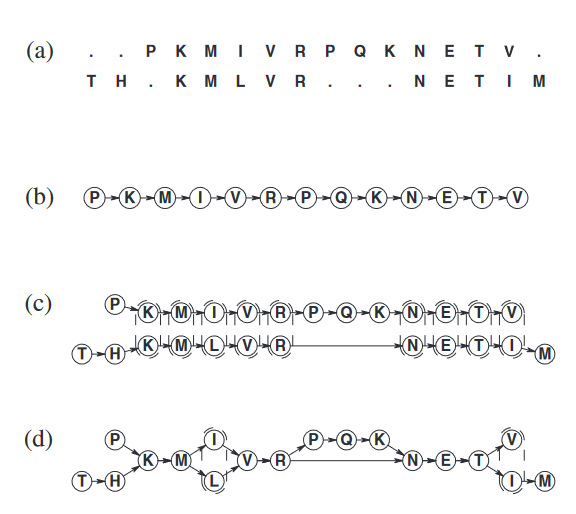
\includegraphics{images/poa-construction.png}
        \caption{\textbf{MSA} rappresentato con un \textbf{POA}. (a) Rappresentazione in formato \textbf{RC-MSA} di un allineamento di sequenze proteiche. (b) Una singola sequenza in formato \textbf{PO-MSA}. (c) Due sequenze proteiche allineate tra loro in formato \textbf{PO-MSA}. I cerchi tratteggiati indicano che due nodi sono allineati. (d) Rappresentazione in formato \textbf{PO-MSA} di un allineamento di due sequenze proteiche. I cerchi tratteggiati indicano che due nodi sono allineati. \cite{POA}}
        \label{fig:poa_construction}
    \end{figure}

\subsubsection{Allineamento tra un POA e una sequenza}
    L'algoritmo di \textbf{programmazione dinamica} \textbf{Needleman-Wunsch} per calcolare l'allineamento tra sequenze (sezione \ref{section:needleman-wunsch}) può essere esteso in maniera da funzionare anche su \textbf{ordini parziali}. In maniera informale, è possibile considerare una sequenza come un grafo degenere, in cui ogni vertice (tranne il primo e l'ultimo) hanno esattamente un predecessore e un successore: per estendere \textbf{Needleman-Wunsch} all'utilizzo di \textbf{POA}, è sufficiente che per ogni vertice non si consideri solo un nodo precedente, bensì tutti i predecessori di tale vertice. Formalmente, considerati in ingresso
    \begin{itemize}
        \item un \textbf{alfabeto} $\Sigma$,
        \item un \textbf{grafo canonico} $G = (V, E, \delta)$ con 
        \begin{itemize}
            \item $V = \{v_1, v_2, ..., v_n\}$ \textbf{ordinato topologicamente}, a cui si aggiunge un vertice $v_0$ per rappresentare il \textbf{grafo vuoto},
            \item $E : V \times V$, a cui si aggiunge $(v_0, v_1)$,
            \item $\delta: V \rightarrow \Sigma$, a cui si aggiunge $\delta(v_0) = \epsilon$,
        \end{itemize}
        \item una \textbf{sequenza (o read)} $X = <x_1, x_2, ..., x_m>, \, x_j \in \Sigma \, \, \forall j \in \{1, 2, ..., m\}$,
        \item una \textbf{matrice di score} $d : (\Sigma \cup \{-\}) \times (\Sigma \cup \{-\}) \rightarrow \mathbb{Q}$
    \end{itemize}
    questo si traduce nella seguente \emph{equazione di ricorrenza}:

    \begin{equation}
        M[v, j] = \max \begin{cases}
            M[u, j] + d(\delta(v), -) & \\
            M[u, j - 1] + d(\delta(v), x_j) & \\
            M[v, j - 1] + d(-, x_j) & \\
        \end{cases}
    \label{equation:poa}
    \end{equation}
    $$\forall u \, s.t. \, (u,v) \in E, \, \forall j > 0 $$

    e nelle seguenti \emph{condizioni al contorno}:
\subsubsection{Caso globale}
    \textbf{Caso base}:
    \begin{equation}
        M[v, j] = \begin{cases}
            0 & v = v_0, \, j = 0 \\
            M[u, 0] + d(\delta(u), -)& \forall (u, v) \in E, \, j = 0 \\
            M[v_0, j - 1] + d(-, x_j)& v = v_0, \, j > 0
        \end{cases}
    \end{equation}

    \textbf{Soluzione ottima}: $$M[v_n, m]$$
    
\subsubsection{Caso semiglobale}
    \textbf{Caso base}:
    \begin{equation}
        M[v, j] = \begin{cases}
            0 & \forall v \in V, \, j = 0 \\
            M[v_0, j - 1] + d(-, x_j) & v = v_0, \, j > 0
        \end{cases}
    \end{equation}
    \textbf{Soluzione ottima}:
    $$\max_{v \in V} M[v, m]$$

\clearpage
\subsubsection{Esempio}
    Come esempio si propone una visualizzazione grafica della \emph{matrice di programmazione dinamica} costruita tramite l'algoritmo appena descritto:
    \begin{figure}[ht]
        \centering
        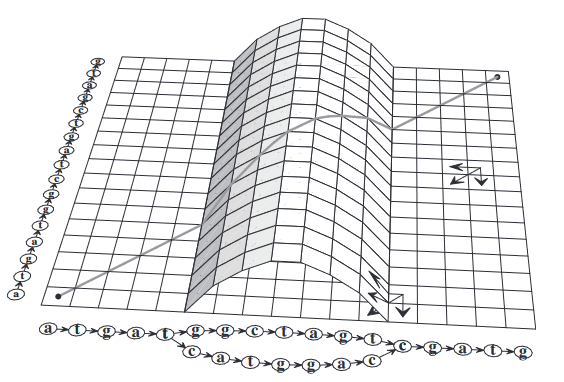
\includegraphics{images/poa-example.png}
        \caption{\emph{Matrice di prgrammazione dinamica} di un allineamento tra un \textbf{POA} e una \textbf{sequenza}. \cite{POA}}
        \label{fig:poa_example}
    \end{figure}
    
    \vspace{20pt}
    Come si vede dalla figura \ref{fig:poa_example}, da ogni \textbf{vertice} con \emph{successori multipli} viene computata una nuova \emph{matrice di programmazione dinamica}; in maniera analoga, in ogni \textbf{nodo} con \emph{più di un predecessore}, due diverse \emph{matrici} si fondono in una sola.  

\subsubsection{Complessità computazionale}
\label{section:poa-complexity}
    Come nell' \textbf{allineamento di sequenze} (sezione \ref{section:needleman-wunsch_complexity}), è necessario computare una matrice di dimensione $(n + 1) \times (m+1)$; la differenza risiede nel fatto che ogni elemento della matrice non è più computabile da un \emph{numero finito} di \emph{casi}, bensì dipende dal numero di \emph{predecessori} di ogni vertice (equazione \ref{equation:poa}): di conseguenza, non è più possibile considerare \emph{costante} il tempo con cui calcola ogni cella. Quindi, definito
    \begin{itemize}
        \item $\bar{n_p}$ = \emph{numero medio} di \emph{predecessori} per vertice
    \end{itemize}
    La \textbf{complessita in tempo} dell'algoritmo risulta essere
    \begin{equation*}
        T(n, m) = \Theta((2\bar{n_p} + 1) \cdot n \cdot m) = \Theta(\bar{n_p} \cdot n \cdot m)
    \end{equation*}
    lineare nel numero di \emph{predecessori} di ogni vertice.
    
    In particolare si noti che, fissando $\bar{n_p}$ a 1, ci si riconduce all'allineamento di due sequenze, con la stessa \textbf{complessità temporale}
    \begin{equation*}
        T(n, m) = \Theta(3 n m) = \Theta(n m)
    \end{equation*}

    Per quanto riguarda la \textbf{complessità in spazio}, ogni elemeneto della matrice continua a mantenere una quantità \emph{costante} di informazione: di conseguenza, essa rimane
    \begin{equation*}
        M(n, m) = \Theta(n m)
    \end{equation*}
    
\subsection{Grafi di variazione}
\label{section:variation_graph}
    Un \textbf{grafo di variazione} (o \textbf{variation graph}) è un'ulteriore generalizzazione dei \textbf{grafi di sequenza}, che permette di rappresentare ancora con maggior efficacia genomi simili contenenti variazioni al loro interno: infatti, nei \textbf{grafi di variazione}, tutte le informazioni sugli aplotitipi sono rappresentate come \emph{percorsi distinti}, mentre nei \textbf{grafi di sequenza} non esiste distinzione sui diversi cammini. Questo è possibile in seguito all'aggiunta di una nuova componente del grafo, ovvero l'insieme di tutti i cammini e dei nodi che li compongono: in questa maniera, ogni variazione è rappresentata da un percorso diverso del grafo, che preso individualmente risulta "lineare" (ogni vertice al suo interno possiede soltanto un predecessore e un successore). Per fare in modo che tutti i cammini inizino e finiscano nello stesso nodo, vengono aggiunti un vertice iniziale e un vertice finali fittizi, appartenenti a tutti i cammini. Da punto di vista matematico, questo si traduce come segue:

    \vspace{20pt}
    \textbf{Definizione}: un \emph{grafo di variazione} è una quadrupla $G = (V, E, \delta, P)$, dove:
    \begin{itemize}
        \item $V = \{v_0, v_1, v_2, ..., v_n\}$ è l'insieme dei \textbf{vertici} del grafo;
        \item  $E \subseteq V \times V$ è l'insieme degli \textbf{archi} del grafo;
        \item $\delta: V \rightarrow \Sigma^*$ è la \textbf{funzione di etichettatura}, che associa a ogni vertice la sequenza corrispondente, 
        \item $P = \{p_1, p_2, ..., p_k\}, \, p_i = <v_0 = v_{i_1}, v_{i_2}, ..., v_{i_l} = v_n> \, \forall i \in \{1, 2, ..., k\}$ è l' \textbf{insieme dei percorsi del grafo}. 
    \end{itemize}
    Anche per i \textbf{grafi di variazione}, se a ogni vertice viene associato un solo carattere (\textbf{funzione di etichettatura} definita come $\delta : V \rightarrow \Sigma$), il \emph{grafo} viene detto \emph{canonico}.
\clearpage
    \begin{figure}[ht]
        \centering
        \begin{tikzpicture}
              % Nodi
              \node[draw, circle] (0) at (5, 1) {$\epsilon$};
              \node[draw, circle] (1) at (5,0) {A};
              \node[draw, circle] (2) at (2,-1.5) {T};
              \node[draw, circle] (3) at (8,-1.5) {A};
              \node[draw, circle] (4) at (2,-3) {C};
              \node[draw, circle] (5) at (4,-3) {G};
              \node[draw, circle] (6) at (8,-3) {G};
              \node[draw, circle] (7) at (8,-4.5) {C};
              \node[draw, circle] (8) at (5, -1.5) {G};
              \node[draw, circle] (10) at (10, -3) {T};
              \node[draw, circle] (12) at (5, -4.5) {$\epsilon$};
            
              % Archi
              \draw[red, ->] (0) to[out=180, in=180] (1);
              \draw[green, ->] (0) to[out=225, in=135] (1);
              \draw[orange, ->] (0) to[out=270, in=90] (1);
              \draw[blue, ->] (0) to[out=315, in=45] (1);
              \draw[brown, ->] (0) to[out=0, in=0] (1);

              \draw[green, ->] (1) -- (2);
              \draw[red, ->] (1) to[out=195, in=90] (2);
              \draw[blue, ->] (1) -- (3);
              \draw[brown, ->] (1) to[out=0, in=135] (3);
              \draw[orange, ->] (1) -- (8);
              \draw[orange, ->] (8) -- (6);
              \draw[red, ->] (2) -- (4);
              \draw[green, ->] (2) -- (5);
              \draw[blue, ->] (3) -- (6);
              \draw[blue, ->] (6) -- (7);
              \draw[orange, ->] (6) to[out=270, in=135] (7);
              \draw[brown, ->] (3) -- (10);
              \draw[brown, ->] (10) -- (7);
              \draw[blue, ->] (7) -- (12);
              \draw[brown, ->] (7) to[out=195, in=345] (12);
              \draw[orange, ->] (7) to[out=165, in=15] (12);
              \draw[red, ->] (4) -- (12);
              \draw[green, ->] (5) -- (12);
              
            \label{graph:variation-graph}
        \end{tikzpicture}
        \caption{Esempio di \textbf{grafo di variazione canonico}: ogni \emph{percorso} è rappresentato da un colore diverso.}
    \end{figure}

\subsection{Allineamento tra un grafo di variazione e una sequenza}
    E' possibile estendere ulteriormente le equazione di \textbf{Needleman-Wunsch} generalizzate a \textbf{grafi di sequenza} (\ref{equation:poa}) per adattarle all'utilizzo di \textbf{grafi di variazione}. In particolare, è necessario aggiungere un'ulteriore dimensione alla \emph{matrice di programmazione dinamica}, in modo da poter riuscire a memorizzare l'allineamento ottimo per ciascun cammino. Considerando un \textbf{grafo di variazione} $G = (V, E, \delta, P)$, questo viene espresso tramite le seguenti \emph{equazioni}:
     \begin{equation}
        M[v, j, p] = \max \begin{cases}
            M[u, j, p] + d(\delta(v), -) & \\
            M[u, j - 1, p] + d(\delta(v), x_j) & \\
            M[v, j - 1, p] + d(-, x_j) & \\
        \end{cases}
    \label{equation:variation-graph}
    \end{equation}
    $$\forall u \, s.t. \, (u,v) \in E, \, \forall j > 0, \, \forall p \in P $$
    \vspace{10pt}
     e dalle seguenti \emph{condizioni al contorno}:
\subsubsection{Caso globale}
    \textbf{Caso base}:
    \begin{equation}
        M[v, j, p] = \begin{cases}
            0 & v = v_0, \, j = 0 \\
            M[u, 0, p] + d(\delta(u), -)& \forall (u, v) \in E, \, j = 0 \\
            M[v_0, j - 1, p] + d(-, x_j)& v = v_0, \, j > 0
        \end{cases}
    \end{equation}
    $$\forall p \in P$$

    \textbf{Soluzione ottima}: $$\max_{p \in P} M[v_n, m, p]$$
    
\subsubsection{Caso semiglobale}
    \textbf{Caso base}:
    \begin{equation}
        M[v, j, p] = \begin{cases}
            0 & \forall v \in V, \, j = 0 \\
            M[v_0, j - 1, p] + d(-, x_j) & v = v_0, \, j > 0
        \end{cases}
    \end{equation}
    \textbf{Soluzione ottima}:
    $$\max_{v \in V, \, p \in P} M[v, m, p]$$

\subsubsection{Esempio}
A seguire un esempio grafico dell'\emph{allineamento} tra un \textbf{grafo di variazione} e una \textbf{sequenza}:
\begin{figure}[ht]
        \centering
        \begin{tikzpicture}
              % Nodi
              \node[draw, circle] (0) at (5, 1) {$\epsilon$};
              \node[draw, circle] (1) at (5,0) {A};
              \node[draw, circle] (2) at (2,-1.5) {T};
              \node[draw, circle] (3) at (8,-1.5) {A};
              \node[draw, circle] (4) at (2,-3) {C};
              \node[draw, circle] (5) at (4,-3) {G};
              \node[draw, circle] (6) at (8,-3) {G};
              \node[draw, circle] (7) at (8,-4.5) {C};
              \node[draw, circle] (8) at (5, -1.5) {G};
              \node[draw, circle] (10) at (10, -3) {T};
              \node[draw, circle] (12) at (5, -4.5) {$\epsilon$};

              \node[draw, circle] (x0) at (13, 1) {-};
              \node[draw, circle] (x1) at (13, 0) {A};
              \node[draw, circle] (x2) at (13, -1.5) {A};
              \node[draw, circle] (x3) at (13, -3) {G};
              \node[draw, circle] (x4) at (13, -4.5) {T};
              \node[draw, circle] (x5) at (13, -6) {-};
            
              % Archi
              \draw[red, ->] (0) to[out=180, in=180] (1);
              \draw[green, ->] (0) to[out=225, in=135] (1);
              \draw[orange, ->] (0) to[out=270, in=90] (1);
              \draw[blue, ->] (0) to[out=315, in=45] (1);
              \draw[brown, ->] (0) to[out=0, in=0] (1);

              \draw[green, ->] (1) -- (2);
              \draw[red, ->] (1) to[out=195, in=90] (2);
              \draw[blue, ->] (1) -- (3);
              \draw[brown, ->] (1) to[out=0, in=135] (3);
              \draw[orange, ->] (1) -- (8);
              \draw[orange, ->] (8) -- (6);
              \draw[red, ->] (2) -- (4);
              \draw[green, ->] (2) -- (5);
              \draw[blue, ->] (3) -- (6);
              \draw[blue, ->] (6) -- (7);
              \draw[orange, ->] (6) to[out=270, in=135] (7);
              \draw[brown, ->] (3) -- (10);
              \draw[brown, ->] (10) -- (7);
              \draw[blue, ->] (7) -- (12);
              \draw[brown, ->] (7) to[out=195, in=345] (12);
              \draw[orange, ->] (7) to[out=165, in=15] (12);
              \draw[red, ->] (4) -- (12);
              \draw[green, ->] (5) -- (12);

              \draw[dashed] (x0) to[out=165, in=90] (0);
              \draw[dashed] (x1) -- (1);
              \draw[dashed] (x2) -- (3);
              \draw[dashed] (x3) to[out=180, in=45] (6);
              \draw[dashed] (x4) -- (7);
              \node (x) at (10.5, -4.5) {\textbf{X}};
              \draw[dashed] (x5) to[out=165, in=270] (12);
              
            \label{graph:variation-graph-alignment}
        \end{tikzpicture}
        \caption{Esempio di allineamento tra un \textbf{grafo di variazione canonico} e una \textbf{sequenza}: il \emph{percorso ottimale} risulta essere quello blu.}
    \end{figure}
\subsubsection{Complessità computazionale}
\label{section:variation-complexity}
   A differenza dell'allineamento con un \textbf{grafo di sequenza} (sezione \ref{section:poa-complexity}), ogni vertice possiede un unico \emph{predecessore} e quindi, sebbene non immediatamente evidente dall'equazione \ref{equation:variation-graph}, ogni cella della matrice viene computata in $O(1)$ (come nell'allineamento tra sequenze). E' tuttavia necessario aggiungere la dimensione relativa ai \emph{percorsi} del grafo alla stessa matrice, che dunque assume una dimensione totale $(n+1) \times (m+1) \times k$, dove $k = \lvert P \rvert$. Di conseguenza, la \textbf{complessità in tempo} risulta essere:
    \begin{equation*}
        T(n, m, k) = O(n \cdot m \cdot k)
        \label{equation:variation_time_complexity}
    \end{equation*}
    
    Per quanto riguarda la \textbf{complessità in spazio}, ogni elemeneto della matrice continua a mantenere una quantità \emph{costante} di informazione: di conseguenza, essa è uguale a
    \begin{equation*}
        M(n, m, k) = O(n \cdot m \cdot k)
    \end{equation*}

\section{Allineamento con ricombinazione}
    Uno dei processi biologici che viene osservato con molta frequenza durante le fasi di duplicazioni del DNA sono le \textbf{ricombinazioni}, le quali consistono nell'importazione totale o parziale di geni al posto di materiale genetico presente in regioni omologhe a quelle importate del genoma di interesse. Uno degli organismi in cui risulta più interessante lo studio delle ricombinazioni sono i \emph{batteri}, nei quali questi processi avvengono con elevate frequenze: esse sono infatti state notate per la prima volta durante lo studio dei emph{loci batterici} che codificano per \emph{antigeni} o per \emph{resistenze agli antibiotici}.
    
    \vspace{20pt}
    Risulta interessante un approccio computazionale che estenda l'allineamento tra un \textbf{grafo di variazione} e una \textbf{sequenza} per riuscire a individuare una, o eventualmente più \textbf{ricombinazioni} avvenute all'interno del genoma rappresentato nel grafo: una trattazione approfondita dell'argomento è riportata in \cite{Recgraph}, mentre di seguito vengono riportate le idee principali dietro a questo tipo di allineamento.

\subsection{Definizioni}
    Si considera un \textbf{grafo di variazione canonico} $G = <V, E, \delta, P>$ (sezione \ref{section:variation_graph});
    
    si definiscono:
    \begin{itemize}
        \item una \textbf{ricombinazione} di \textbf{due percorsi} come una quadrupla $R = <p_1, p_2, \rho, \psi>$, dove 
            \begin{itemize}
                \item $p_1, p_2 \in P$ sono due \emph{cammini} del grafo;
                \item $\rho \in p_1$ e $\psi \in p_2$ sono due \emph{vertici} dei cammini selezionati.
            \end{itemize}

        \item i due vertici\footnote{Quando chiari dal contesto, i cammini $p_1, p_2$ e i vertici $\rho, \psi$ vengono omessi e i vertici indicati come $\alpha$ e $\beta$.} $\alpha_{p1, p2}(\rho, \psi) \in V$ e $\beta_{p1, p2}(\rho, \psi) \in V$ come due nodi per i quali:
        \begin{itemize}
            \item $\alpha_{p1, p2}(\rho, \psi)$ precede $\rho$ in $p_1$ e $\psi$ in $p_2$, e segue qualsiasi altro vertice $u$ che precede entrambi $\rho$ in $p_1$ e $\psi$ in $p_2$;
            \item $\beta_{p1, p2}(\rho, \psi)$ segue $\rho$ in $p_1$ e $\psi$ in $p_2$, e precede qualsiasi altro vertice $v$ che segue entrambi $\rho$ in $p_1$ e $\psi$ in $p_2$;
        \end{itemize}
        ricordando il concetto \emph{Lower Common Ancestor (LCA)} di un albero;

        \item il \textbf{displacement di una ricombinazione} come la quantità 
        \begin{equation}
            D = \lvert \lvert a_1 \rvert - \lvert a_2 \rvert + 1 \rvert + \lvert \lvert b_1 \rvert - \lvert b_2 \rvert - 1 \rvert 
            \label{equation:displacement}
        \end{equation}
        dove:
        \begin{itemize}
            \item $a_1, \, a_2$ sono i \emph{sottopercorsi} che vanno rispettivamente da $\alpha$ a $\rho$ e da $\alpha$ a $\psi$;
            \item $b_1, \, b_2$ sono i \emph{sottopercorsi} che vanno rispettivamente da $\rho$ a $\beta$ e da $\psi$ a $\beta$;
        \end{itemize}
        che vuole misurare il \emph{peso} di una \textbf{ricombinazione};

        \item un \textbf{allineamento con ricombinazione} come la concatenazione di due allineamenti senza ricombinazione:
        \begin{itemize}
            \item il primo che riguarda il \emph{sottopercorso} $a_1$ e il \emph{prefisso} $Y[:j]$,
            \item il secondo che riguarda il \emph{sottopercorso} $b_2$ e il \emph{suffisso} $Y[j+1:]$,
        \end{itemize}
        dove $Y_m$ è la sequenza da allineare e $j \in \{1, ..., m\}$ la posizione della sequenza in cui avviene la \textbf{ricombinazione}. 
    \end{itemize}

    Un esempio delle definizioni introdotte è mostrato nella figura \ref{fig:recombination_definitions_example}.

    \vspace{20pt}
    \begin{figure}[H]
        \centering
        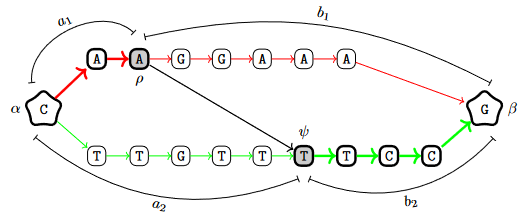
\includegraphics[width=1.0\linewidth]{images/recombination_definitions_example.png}
        \caption{Esempio di \textbf{displacement} di una \textbf{ricombinazione}. \cite{Recgraph}}
        \label{fig:recombination_definitions_example}
    \end{figure}

\subsection{Equazioni di ricorrenza}
    Come conseguenza della definizione, un \textbf{allineamento con ricombinazione} può essere computato attraverso due diversi \textbf{allineamenti senza ricombinazione}, uno che comprenda la porzione iniziale di un cammino e il prefisso della read e l'altro che si riferisca alla porzione finale di un altro cammino e al suffisso della stessa read.

    Formalmente, definita $M[v, j, p]$ come in \ref{equation:variation-graph} e $R[v, j, p]$ come il valore ottimale dell'allineamento globale tra la porzione finale di $p \in P$ che inizia nel vertice $\psi$ e tra il \emph{suffisso} $Y[:j]$, il valore ottimale dell'\textbf{allineamento con al più una ricombinazione} può essere descritto dalla ricorrenza \ref{equation:recombination}:

    \begin{equation}
        \max {\begin{cases}
            \max_{p \in P}{M[v_0, m, p]} & (a) \\
            \max_{(v, w), j, p \neq q}{M[v, j, p] + R[w, j+1, q] + d_o + d_e \cdot d(v,w)} & (b) \\
        \end{cases}}
        \label{equation:recombination}
    \end{equation}
    dove:
    \begin{itemize}
        \item $d(v, w)$ è il \textbf{displacement} tra $v$ e $w$ (equazione \ref{equation:displacement});
        \item $d_o$ è il \textbf{costo di apertura} del \textbf{displacement};
        \item $d_e$ è il \textbf{costo di estensione} del \textbf{displacement};
    \end{itemize}

    Se il massimo è verificato dal caso $(a)$, allora l' \emph{allineamento ottimale} è \textbf{senza ricombinazione}; se invece è verificato dal caso $(b)$, si trova un \textbf{allineamento con una ricombinazione}.

    \vspace{20pt}
    \begin{figure}[H]
        \centering
        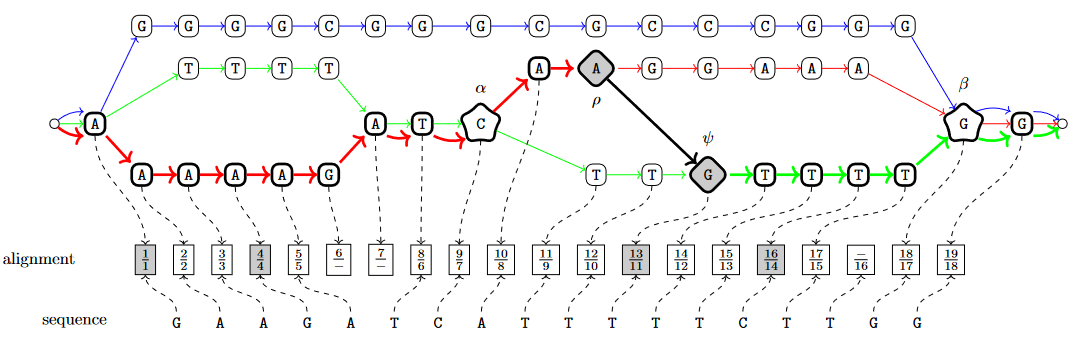
\includegraphics[width=1 \linewidth]{images/recombination_alignment.png}
        \caption{Esempio di un \textbf{allineamento ottimale con ricombinazione}. \cite{Recgraph}}
        \label{fig:recombination_alignment}
    \end{figure}
    

\subsection{Complessità computazionale}
\subsubsection{Complessità in tempo}
    La \textbf{complessità temporale} per computare le due matrici $M[v, j, p]$ e $R[v, j, p]$ rimane la stessa di \ref{equation:variation_time_complexity} (le due matrici possono anche essere calcolate in parallelo); di conseguenza, definiti
    \begin{itemize}
        \item $n = \lvert V \rvert$
        \item $m = \lvert Y \rvert$
        \item $p = \lvert P \rvert$
    \end{itemize}
    la \textbf{complessità in tempo} è data dal caso $(b)$ dell'equazione \ref{equation:recombination} e vale:

    \begin{equation}
        T(n, m, p) = O(n^2 \cdot m \cdot p^2)
        \label{equation:recombination_time_complexity}
    \end{equation}

\subsubsection{Complessità in spazio}
    Le due matrici $M[v, j, p]$ e $R[v, j, p]$ occupano la stessa quantità di memoria; di conseguenza la \textbf{complessità in spazio} rimane:

    \begin{equation}
        M(n, m, p) = O(n \cdot m \cdot p)
        \label{equation:recombination_space_complexity}
    \end{equation}

\subsection{RecGraph}
\label{section:recgraph}
    \href{https://github.com/AlgoLab/RecGraph}{\textbf{\textit{RecGraph}}} è un tool sviluppato dal laboratorio \href{https://algolab.eu/}{\textbf{BIAS}}, nel linguaggio di programmazione \href{https://www.rust-lang.org/it}{\textbf{\textit{Rust}}}, che permette di eseguire allineamenti tra un \textbf{grafo} e una \textbf{sequenza} in diverse modalità, tra cui la \textbf{\textit{recombination mode}}, in cui si cerca di individuare fino a una \textbf{ricombinazione} avvenuta nel genoma corrispondente a uno dei percorsi del grafo. Un'interessante ottimizzazione per l'allineamento su \textbf{grafi di variazione} implementata all'interno del tool è il \textbf{reference path}, che permette di evitare di calcolare più di una volta il valore dell'allineamento di vertici appartenenti a più di un \emph{cammino} (spiegazione formale contenuta in \cite{Recgraph}).    

    \vspace{20pt}
    L'obiettivo finale dello stage era quello di cercare di migliorare le capacità computazionali di \textbf{\textit{RecGraph}}, concentrandosi sull'allineamento tra un \textbf{grafo di variazione} e una \textbf{sequenza}, in maniera che potesse poi essere utilizzato nella \textbf{\textit{recombination mode}} su grafi di dimensioni maggiori (e, in futuro, possa essere usato per permettere più di una ricombinazione): per far questo, si è passati allo studio dell' \textbf{algoritmo \textit{wavefront}}, di cui segue una trattazione formale nel capitolo successivo.
    \chapter{Algoritmo wavefront per la distanza di edit}
    La \textbf{complessità in tempo} (e \textbf{in memoria}) $\Theta(n m)$ rende poco pratico l'utilizzo dell'algoritmo di \textbf{Needleman-Wunsch} \cite{NeedlemanWunsch} su sequenze di grandi dimensioni; ciò risulta ancora più evidente nell'estensione dell'algoritmo sui \textbf{grafi di sequenza} (sezione \ref{section:poa-complexity}) e sui \textbf{grafi di variazione} (sezione \ref{section:variation-complexity}), limitando fortemente le dimensioni dei grafi che è possibile trattare in tempi realistici. Recentemente è stato ripreso e sviluppato \cite{WFA_edit-distance} un algoritmo per calcolare l'allineamento di sequenze in modo esatto, chiamato \textbf{\textit{wavefront algorithm} (WFA)} \cite{UKKONEN1985100}, che permette di computare la \textbf{distanza di edit} di \emph{due sequenze} con una complessità in tempo lineare rispetto alla dimensione delle sequenze e al valore ottimale della stessa \textbf{distanza di edit}: in questo capitolo si propone una trattazione formale dell'algoritmo e una sua possibile estensione sui \textbf{grafi di variazione}. 
\label{section:wfa}

\section{Algoritmo wavefront per la distanza di edit tra due sequenze}
    Quando si calcola la \textbf{distanza di edit} tra due sequenze utilizzando le equazioni descritte nella sezione \ref{section:edit-distance}, la \emph{matrice di programmazione dinamica} di dimensione $(n + 1) \times (m + 1)$ viene computata completamente, indipendentemente da quale sia il valore effettivo della \textbf{distanza di edit ottimale}:
\clearpage

    \begin{figure}[ht]
        \centering
        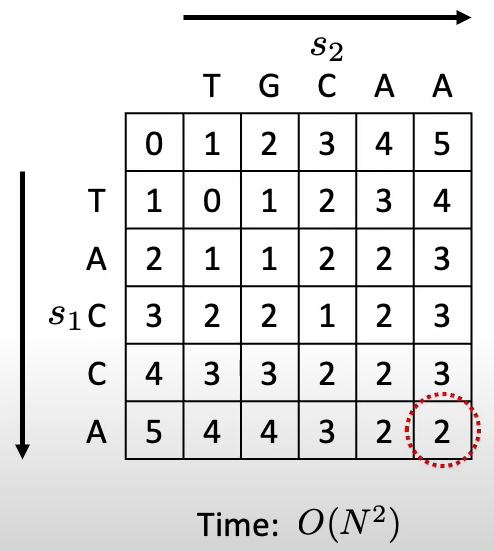
\includegraphics[width=0.5\textwidth]{images/wfa_complete_matrix.png}
        \caption{\emph{Matrice di programmazione dinamica} per il calcolo della \textbf{distanza di edit} tra due sequenze. \cite{wfa_sequence_graph}}
        \label{fig:wfa_complete_matrix}
    \end{figure}
    \vspace{20pt}
    Tuttavia, è possibile notare che tutte le celle che hanno un valore strettamente maggiore della \textbf{distanza di edit ottimale} non contribuiscono al calcolo della soluzione ottimale e, di conseguenza, non si troveranno mai nel percorso che porta alla soluzione migliore. Questa è una conseguenza diretta del fatto che l'algoritmo di programmazione dinamica della \textbf{distanza di edit} risolve un \emph{problema di minimizzazione} in cui le \emph{penalità} utilizzate sono \emph{strettamente positive}: di conseguenza, prese in ingresso le due sequenze $X_n = <x_1, x_2, ..., x_n>$ e $Y_m = <y_1, y_2, ..., y_m>$, vale la seguente proprietà:
    \begin{equation*}
        D[i, j] \geq D[i-1, j-1]
    \end{equation*}
    e, in particolare
    \begin{equation*}
       D[i, j] = D[i-1, j-1] \iff x_i = y_j
    \end{equation*}
    $$\forall i \in \{1, ..., n\}, \, \forall j \in \{1, ..., m\}$$
    Detto a parole, le \emph{diagonali} sono \emph{crescenti in senso lato} su tutta la matrice, e \emph{crescenti in senso stretto} se non sono presenti corrispondenze (\emph{match}) nelle sottostringhe considerate. L'idea dietro all'algoritmo \textbf{\textit{wavefront}} è di sfruttare questa proprietà per evitare di calcolare tutte le celle che corrispondono a una \textbf{distanza di edit} maggiore di quella ottimale: per far questo, gli indici e il contenuto della matrice di programmazione dinamica cambiano come segue:
    \begin{itemize}
        \item gli indici della matrice diventano la \emph{diagonale} che si sta computando e lo \textbf{distanza di edit} a cui si è arrivati;
        \item il valore degli elementi della matrice diventa il maggior \emph{offset} sulla \emph{diagonale} di interesse per la \emph{distanza di edit} considerata.
    \end{itemize}
    Si definisce \textbf{fronte d'onda} l'insieme composto dalle celle della matrice che hanno la stessa \emph{distanza di edit}: esse vengono computate tutte durante la medesima iterazione dell'algoritmo. E' possibile suddividere \textbf{\textit{WFA}} in due fasi principali:
    \begin{itemize}
        \item L'\textbf{estensione}, in cui tutte le diagonali appartenenti allo stesso \emph{fronte d'onda} vengono appunto "estese" il più possibile (fino a quando ci sono dei \textbf{match} tra i simboli delle sequenze); 
        \item L'\textbf{espansione}, in cui viene computato il \emph{fronte d'onda successivo} a partire dalle diagonali del \emph{fronte d'onda attuale}.
    \end{itemize}
    
    \begin{figure}[h]
        \centering
        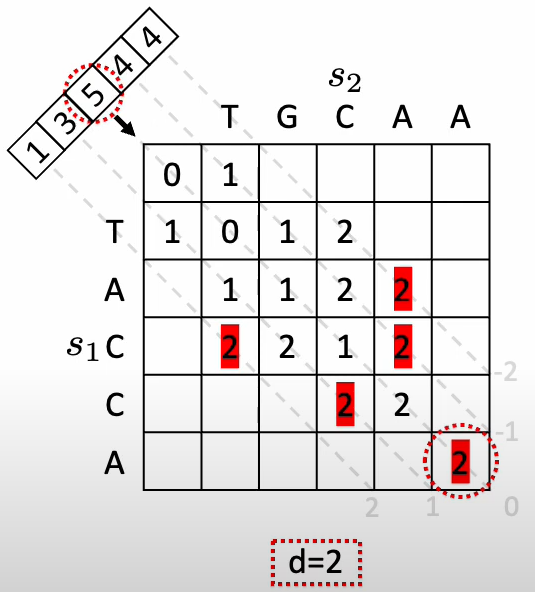
\includegraphics[width=0.5\textwidth]{images/wfa_partial_matrix.png}
        \caption{\emph{Matrice di programmazione dinamica} virtualmente computata da \textbf{\textit{WFA}}: i numeri in basso a destra rappresentano il numero della \emph{diagonale}, mentre quelli in alto a sinistra il valore degli \emph{offset} sulle rispettive \emph{diagonali}. \cite{wfa_sequence_graph}}
        \label{fig:wfa_partial_matrix}
    \end{figure}
    \vspace{20pt}

\subsection{Equazioni di ricorrenza}
    Da un punto di vista matematico, questo viene espresso dalle seguenti equazioni: siano

    \begin{itemize}
        \item $\Sigma$ l'\textbf{alfabeto} di definizione,
        \item  $X_n = <x_1, x_2, ..., x_n>, \, x_i \in \Sigma \, \, \forall i \in \{1, 2, ..., n\}$ la \textbf{prima sequenza},
        \item  $Y_m = <y_1, y_2, ..., y_m>, \, y_j \in \Sigma \, \, \forall j \in \{1, 2, ..., m\}$ la \textbf{seconda sequenza},
        \item $$D[i, j] = \begin{cases}
            D[i-1, j-1] & se \, \, x_i = y_j \\
            \min \begin{cases}
                D[i, j-1] & \\
                D[i-1, j-1] & \\
                D[i-1, j] & \\
            \end{cases} + 1 & se \, \, x_i \neq y_j 
        \end{cases}$$ la \emph{matrice di programmazione dinamica} computata dall'algoritmo standard per il calcolo della \textbf{distanza di edit} (sezione \ref{section:edit-distance});
    \end{itemize}

    Si definiscono
    \begin{itemize}
        \item $k = j - i$ come la \emph{k-esima diagonale},
        \item \begin{equation}
            H[d, k] = \begin{cases}
                max\{j \mid D[j - k, j] = d\}, & \, se \, \, \exists j \, s.t. \, D[j - k, j] = d \\
                -\infty, & altrimenti
            \end{cases}
        \label{equation:wf_extension_definition}
        \end{equation}
        come il valore del maggior \emph{offset} per la \emph{k-esima diagonale} tra le celle di programmazione dinamica con \textbf{distanza di edit} \emph{d} (dopo una fase di \textbf{estensione}).
        \item \begin{equation}
            J[d, k] = \begin{cases}
                min\{j \mid D[j - k, j] = d\}, & \, se \, \, \exists j \, s.t. \, D[j - k, j] = d \\
                -\infty, & altrimenti
            \end{cases}
        \label{equation:wf_expansion_definition}
        \end{equation}
        come il valore del minor \emph{offset} per la \emph{k-esima diagonale} tra le celle di programmazione dinamica con \textbf{distanza di edit} \emph{d} (dopo una fase di \textbf{espansione}).
    \end{itemize}
    Come conseguenza delle definizioni \ref{equation:wf_extension_definition} e \ref{equation:wf_expansion_definition} vale la seguente implicazione:
    \begin{equation*}
        D[j-k, j] = d \iff J[d,k] \leq j \leq H[d,k]
    \end{equation*}
    Ovvero l'\emph{offset} di qualsiasi cella con \textbf{distanza di edit} $d$ che si trova sulla diagonale $k$ è compreso tra  $J[d,k]$ e $H[d,k]$.
    
    Le due fasi di \textbf{estensione} ed \textbf{espansione} vengono descritte dalle seguenti equazioni di ricorrenza:
\subsubsection{Estensione del fronte d'onda}
    \begin{equation}
        H[d,k] = j + LCP(X[j - k + 1:], Y[j + 1:]), \quad j = J[d,k]
    \label{equation:wf-extension}
    \end{equation}
    dove
    $$LCP(x, y) = \lvert Longest \, Common \, Prefix(x, y) \rvert$$

\subsubsection{Espansione del fronte d'onda}
    \begin{equation}
        J[d, k] = max \begin{cases}
            H[d - 1, k - 1] + 1, \\
            H[d - 1, k] + 1, \\
            H[d - 1, k + 1]
        \end{cases}
    \label{equation:wf-expansion}
    \end{equation}

    Le equazioni \ref{equation:wf-extension} e \ref{equation:wf-expansion} esprimono l'alternarsi delle due fasi di \textbf{estensione} ed \textbf{espansione}: dopo aver computato tutti i \textbf{match} possibili, le diagonali vengono espanse per la \textbf{distanza di edit} successiva, per poi reiterare il procedimento.

\subsection{Condizioni al contorno}
    Le \textbf{condizioni al contorno} vengono riformulate come segue:

\subsubsection{Caso globale}
    \textbf{Caso base}:
    \begin{equation}
        H[0, 0] = 0
    \label{section:wfa_global_base_case}
    \end{equation}

    \textbf{Soluzione ottima}: $$d \, \, s.t \, \, H[d, m - n] = m$$
    
\subsubsection{Caso semiglobale}
    \textbf{Caso base}:
    \begin{equation}
        H[0, -i] = 0, \quad \forall i \in \{0, ..., n\} 
        \label{section:wfa_semiglobal_base_case}
    \end{equation}
    \textbf{Soluzione ottima}:
    $$d \, \, s.t \, \, H[d, m - i] = m, \quad \forall i \in \{0, ..., n\}$$

\subsection{Pseudocodice}
    Da un punto di vista algoritmico, le due procedure di \textbf{estensione} ed \textbf{espansione} vengono espresse tramite il seguente pseudocodice:
\subsubsection{Extend}
    \begin{algorithm}[H]
        \KwData{$X_n, Y_m, d, H_d$}
        \For{k = -d \KwTo d} {
            $i \gets H[d][k] - k$\;
            $j \gets H[d][k]$\;
            \While{$x_i = y_j$} {
                $i \gets i + $1\;
                $j \gets j + 1$\;
                $H[d][k] \gets H[d][k] + 1$\;
            }
        }
    \caption{extend}
    \label{alg:extend}
    \end{algorithm}
    Nell'estensione il numero di diagonali del \emph{d-esimo fronte d'onda} non cambia.
    
\subsubsection{Expand}
    \begin{algorithm}[H]
        \KwData{$X_n, Y_m, d, H_d$}
        \textbf{initialize} $H_{d+1}$\;
        $k_{lo} \gets -(d + 1)$\;
        $k_{hi} \gets d + 1$\;
        \For{k = $k_{lo}$ \KwTo $k_{hi}$} {
            $H[d + 1, k] \gets \max\{H[d, k - 1] + 1, \, H[d, k] + 1, \, H[d, k + 1]\}$\;
        }
        \caption{expand}
        \label{alg:wf_expand}
    \end{algorithm}
    Nella fase di espansione viene computato il \emph{fronte d'onda} successivo: è necessario considerare le due nuove diagonali $-(d+1)$ e $d+1$.
    
    \vspace{20pt}
    A seguire lo pseudocodice per la procedura  principale \textbf{\textit{WFA}} nella \textbf{modalità globale}:
\subsubsection{Caso globale}
    \begin{algorithm}[H]
        \caption{WFA\_global}
        \label{alg:wfa_global}
        \KwData{$X_n, Y_m$}
        \KwResult{$d = edit\_distance(X_n, Y_m)$}
        \textbf{initialize} $H_0$\;
        $H[0][0] \gets 0$\;
        $d \gets 0$\;
        \While{$true$}{
            $extend(X_n, Y_m, d, H_d)$\;
            \If{$H[d, m-n] = m$} {
                $break$\;
            }
            $expand(X_n, Y_m, d, H_d)$\;
            $d \gets d + 1$\;
          }
        $traceback(X_n, Y_m, d, H_d)$\;
        $return \, d$\;
    \end{algorithm}

    \vspace{20pt}
    E nella \textbf{modalità semiglobale}:
    
\subsubsection{Caso semiglobale}
    \begin{algorithm}[H]
        \caption{WFA\_semiglobal}
        \label{alg:wfa_semiglobal}
        \KwData{$X_n, Y_m$}
        \KwResult{$d = edit\_distance(X_n, Y_m)$}
        \textbf{initialize} $H_0$\;
        \For{i = 0 \KwTo n} {
            $H[0][-i] = 0$
        }
        $d \gets 0$\;
        \While{$true$}{
            $extend(X_n, Y_m, d, H_d)$\;
            \For{i = 0 \KwTo n} {
                \If{$H[d, m-i] = m$} {
                    $break$\;
                }
            }
            $expand(X_n, Y_m, d, H_d)$\;
            $d \gets d + 1$\;
          }
        $traceback(X_n, Y_m, d, H_d)$\;
        $return \, d$\;
    \end{algorithm}

    Si noti che nella \textbf{modalità semiglobale}, le sottoprocedure \textbf{extend} ed \textbf{expand} vanno modificate in maniera da considerare il range di diagonali $[-n, d]$ a ogni iterazione.
    \vspace{20pt}

    Infine un esempio (figura \ref{fig:wfa-example}) che mostra la \emph{matrice} computata da \textbf{\textit{WFA\_global}} e quella che verrebbe virtualmente calcolata dall'algoritmo standard:
    
    \begin{figure}[ht]
        \centering
        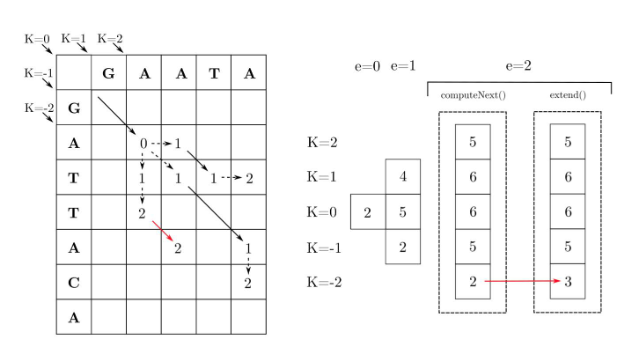
\includegraphics[width=1\textwidth]{images/wfa_example.png}
        \caption{Matrice effettivamente calcolata da \textbf{\textit{WFA}} rispetto a quella che verrebbe virtualmente computata dall'algoritmo standard. \cite{WFA_edit-distance}}
        \label{fig:wfa-example}
    \end{figure}

\subsection{Complessità computazionale}
    Si consideri la seguente notazione:
    \begin{itemize}
        \item $n$ = lunghezza della \emph{sequenza più lunga} \textbf{(testo)},
        \item $m$ = lunghezza della \emph{sequenza più corta} \textbf{(query)},
        \item $\overline{d}$ il valore ottimo della \textbf{distanza di edit} tra le due sequenze.
    \end{itemize}
    Si noti che la \textbf{distanza di edit} $d$ è \emph{limitata inferiormente} dalla differenza della lunghezza delle due sequenze ed è \emph{limitata superiormente} dalla lunghezza maggiore tra le sequenze:
    \begin{equation}
        n - m \leq \overline{d} \leq n
    \label{equation:edit-dist_limit}
    \end{equation}

\subsubsection{Complessità in tempo}
    La \textbf{complessità in tempo} di \textbf{\textit{WFA}} è determinata dalle operazioni presenti all'interno del ciclo principale, che viene eseguito una volta per ogni valore della \textbf{distanza di edit} $d \in \{0, 1, ..., \overline{d}\}$ e contenente le tre sottoprocedure:
    \begin{itemize}
        \item \textbf{extend},
        \item \textbf{controllo terminazione},
        \item \textbf{expand},
    \end{itemize}
    e dalla procedura \textbf{traceback}. Si procede a analizzare il tempo richiesto da ognuna delle sottoprocedure.
\subsubsection{Extend}
\begin{itemize}
    \item \textbf{Caso globale}: nella sottoprocedura \textbf{extend} (algoritmo \ref{alg:extend}) il tempo di esecuzione è proporzionale al numero totale di \textbf{match} effettuato da tutte le diagonali, appartenenenti all'insieme $\{-\overline{d}, -\overline{d} + 1, ..., 0, ..., \overline{d}-1, \overline{d}\}$.
        E' possibile distinguere due casi:
        \begin{itemize}
            \item $m \leq \overline{d} \leq n \implies m = O(\overline{d})$, rappresentato dalla seguente figura
            \vspace{20pt}
                \begin{figure}[h]
                    \centering
                    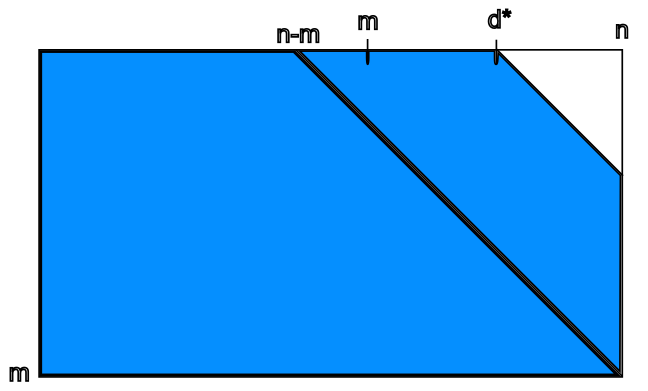
\includegraphics[width=0.7\textwidth]{images/wfa_extend_matrix_1.png}
                    \caption{Sezione della \emph{matrice di programmazione dinamica} in cui si possono verificare il massimo numero di \textbf{match} (caso $m \leq \overline{d} \leq n$).}
                    \label{fig:wf_extend_matrix_1}
                \end{figure}
    
                In questo caso il \emph{numero massimo} di \textbf{match} è dato da
                \begin{align*}
                    &T(n, m, \overline{d}) = \\ 
                    &= \sum_{j=0}^{m}{m-j}& &+& &\sum_{i=1}^{n-m}{m}& &+& &\sum_{i=1}^{\overline{d}-(n-m)}{m-i} = \\
                    &= \frac{m(m+1)}{2}& &+& &m(n-m)& &+& &\frac{(\overline{d}-(n-m)) (m+(n-\overline{d})-1)}{2}
                \end{align*}
                Per \ref{equation:edit-dist_limit} si ha che
                \begin{itemize}
                    \item $n-m \leq \overline{d} \implies n-m = O(\overline{d})$
                    \item  $n - \overline{d} \leq m \implies n-\overline{d} = O(m)$
                \end{itemize}
                e di conseguenza
                \begin{align*}
                    T(n, m, \overline{d}) = O(m^2) + O(m) \cdot O(\overline{d}) + O(\overline{d}) \cdot O(m) = O(m \cdot \overline{d})
                \end{align*}
                Si osservi che porre $n-m \leq m \leq \overline{d}$ non è limitante, in quanto è il caso in cui si considerano il maggior numero di diagonali (rispetto al caso $m \leq n-m \leq \overline{d}$ o al caso $m \leq \overline{d} \leq n-m$).
            
            \item $\overline{d} \leq m \leq n \implies m = O(\overline{d})$, rappresentato dalla seguente figura
            \vspace{20pt}
                \begin{figure}[h]
                    \centering
                    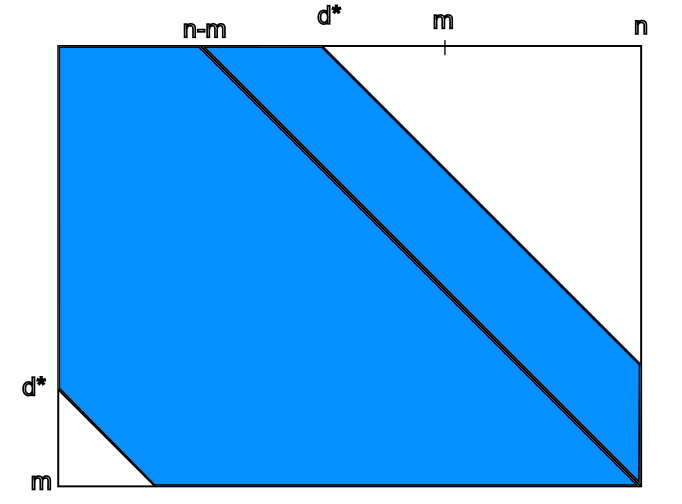
\includegraphics[width=0.7\textwidth]{images/wfa_extend_matrix_2.png}
                    \caption{Sezione della \emph{matrice di programmazione dinamica} in cui si possono verificare il massimo numero di \textbf{match} (caso $\overline{d} \leq m \leq n$).}
                    \label{fig:wf_extend_matrix_2}
                \end{figure}
                
                Per questa altra possibilità si nota che viene computata una sezione di \emph{matrice di programmazione dinamica} inferiore rispetto al caso precedente; quindi il tempo sarà sempre limitato da
                $$T(n, m, \overline{d}) = O(m \cdot \overline{d})$$
                Anche in questa casistica, porre $n-m \leq \overline{d} \leq m$ non è limitante.
        \end{itemize}
        Quindi, il tempo della sottoprocedura \textbf{extend} nel \textbf{caso globale} è \emph{limitato superiormente} da
        $$T(n, m, \overline{d}) = O(\min\{n, m\} \cdot \overline{d})$$
        
    \item \textbf{Caso semiglobale}: in questa modalità, vengono considerate tutte le diagonali $k \in \{0, -1, ..., -n\}$      fin dalla prima iterazione; di conseguenza, il tempo di esecuzione risulta:
        \begin{align*}
                    &T(n, m, \overline{d}) = \\ 
                    &= \sum_{j=0}^{\overline{d}}{m-j}& &+& &\sum_{i=1}^{n-m}{m}& &+& &\sum_{i=1}^{n-(n-m)}{m-i} = \\
                    &= \frac{(\overline{d}+1) \cdot (2m -\overline{d})}{2}& &+& &m(n-m)& &+& &\frac{m(m-1)}{2}
                \end{align*}
        ovvero
        \begin{equation*}
            T(n, m, \overline{d}) = O(m \cdot (\overline{d} + m))
        \end{equation*}
         
    \end{itemize}

\subsubsection{Controllo terminazione}
    \begin{itemize}
        \item Per quanto riguarda il \textbf{caso globale} (algoritmo \ref{alg:wfa_global}), il \textbf{controllo di terminazione} viene effettuato in tempo costante: 
        $$T(n, m, \overline{d}) = O(1)$$
        \item Nel \textbf{caso semiglobale} (algoritmo \ref{alg:wfa_semiglobal}), invece, è necessario controllare a ogni iterazione gli offset di tutte le diagonali corrispondenti a una posizione della sequenza più lunga (chiamata \textbf{testo}); il tempo risulta quindi essere 
        $$T(n, m, \overline{d}) = O(\max\{n, m\} \cdot \overline{d})$$ 
    \end{itemize}

\subsubsection{Expand}
    \begin{itemize}
        \item \textbf{Caso globale}: nella sottoprocedura \textbf{expand} (algoritmo \ref{alg:wf_expand}) ad ogni iterazione vengono effettuate $O(2d+1)$ operazioni: di conseguenza, la complessità temporale risulta essere limitata da $O(\sum_{d=0}^{\overline{d}}{2d+1}) = O(\overline{d} \cdot (\overline{d}+2)) = O(\overline{d}^2)$, ovvero:
        $$T(n, m, \overline{d}) = O(\overline{d}^2)$$

        \item \textbf{Caso semiglobale}: come succede nella \textbf{extend}, anche qui è necessario considerare tutte le diagonali $k \in \{0, -1, ..., -n\}$ fin dalla prima iterazione; il tempo risulta quindi $O(\sum_{d=0}^{\overline{d}}{d+n}) = O(\max\{n, m\} \cdot \overline{d}) + O(\overline{d}^2)$, ossia
        \begin{equation*}
            T(n, m, \overline{d}) = O(\max\{n, m\} \cdot \overline{d})
        \end{equation*}
    \end{itemize}
   

\subsubsection{Traceback}
    Come nel calcolo della \textbf{distanza di edit} standard, il tempo richiesto per ricostruire la soluzione è
    $$T(n, m, \overline{d}) = O(n + m)$$
    per entrambe le modalità.
    
    \vspace{20pt}
    La \textbf{complessità in tempo} totale risulta quindi essere:
    \begin{itemize}
        \item \textbf{Caso globale}:
        \begin{align*}
            T(n, m, \overline{d}) &= O(\min\{n, m\} \cdot \overline{d} + O(1) + O(\overline{d}^2) + O(n + m)) = \\
                                  &= O(\min\{n, m\} \cdot \overline{d} + \overline{d}^2 + (n + m))
        \end{align*}
        se interessati anche alla \textbf{ricostruzione della soluzione}, altrimenti
        \begin{equation}
            T(n, m, \overline{d}) = O(\min\{n, m\} \cdot \overline{d} + \overline{d}^2)
            \label{equation:wfa_global_time_complexity}
        \end{equation}
        \item \textbf{Caso semiglobale}:
        \begin{equation*}
            T(n, m, \overline{d}) = O(m \cdot (m + \overline{d})) + 2 \cdot O( \max\{n, m\} \cdot \overline{d}) + O(n + m)
        \end{equation*}
        ossia
        \begin{equation}
            T(n, m, \overline{d}) = O(\max\{n, m\} \cdot \overline{d})
             \label{equation:wfa_semiglobal_time_complexity}
        \end{equation}
    \end{itemize}

\subsubsection{Complessità in spazio}
    \begin{itemize}
        \item \textbf{Caso globale}: per quanto riguarda la \textbf{complessità in spazio}, ogni \emph{fronte d'onda} ha una dimensione proporzionale a $2d + 1$, con $d$ che varia da 0 a $\overline{d}$; di conseguenza, la \textbf{complessità spaziale}\footnote{Se non interessati alla \textbf{ricostruzione della soluzione}, la complessità scende a $M(n, m, \overline{d}) = O(\overline{d})$.} nel \textbf{caso globale} è data da
        \begin{equation}
            M(n , m, \overline{d}) = O(\overline{d}^2)
        \label{equation:wfa_global_space_complexity}
        \end{equation}

        \item \textbf{Caso semiglobale}: in questa modalità, vale la stessa osservazione del \textbf{caso globale}; tuttavia, è necessario considerare anche le diagonali $k \in \{0, -1, ..., -n\}$ fin dalla prima iterazione. La \textbf{complessità in spazio}\footnote{Se non interessati alla \textbf{ricostruzione della soluzione}, la complessità scende a $M(n, m, \overline{d}) = O(\max\{n, m\})$.} diventa quindi limitata da $O(\sum_{d=0}^{\overline{d}}{d+n}) = O(\max\{n, m\} \cdot \overline{d}) + O(\overline{d}^2)$, e di conseguenza
        \begin{equation}
            M(n , m, \overline{d}) = O(\max\{n, m\} \cdot \overline{d})
        \label{equation:wfa_semiglobal_space_complexity}
        \end{equation}
        
    \end{itemize}
    

\subsection{Dimostrazione di correttezza}
    Si considerino due \textbf{sequenze} $X_n = <x_1, x_2, ..., x_n>$ e $Y_m = <y_1, y_2, ..., y_m>$; la \textbf{distanza di edit} tra qualsiasi coppia di \textbf{prefissi} $X[:i]$, $Y[:j]$ è descritta dalla seguente equazione
    
    \begin{equation*}
        D[i,j] = \min \begin{cases}
            D[i-1,j] + 1 \\
            D[i-1,j-1] + \Delta_{i,j} \\
            D[i,j-1] + 1 \\
        \end{cases}
    \end{equation*}
    
    $$\Delta_{i,j} = \begin{cases}
        0 & \text{se }x_i = y_j \\
        1 & altrimenti
    \end{cases}$$
    che è \textbf{equivalente} alle seguenti equazioni
    
    \begin{equation}
        J[d,k] = \max \begin{cases}
            H[d-1, k + 1] \\
            H[d-1, k] + 1 \\
            H[d-1, k - 1] + 1 \\
        \end{cases}    
        \label{equation:expansion_demonstration}
    \end{equation}
        
    \begin{equation}
        H[d, k] = j + LCP(X[j - k + 1:], Y[j + 1:]), \quad j = J[d, k]
        \label{equation:extension_demonstration}
    \end{equation}
    con
    $$LCP(X, Y) = \lvert Longest \, Common \, Prefix (X, Y) \rvert$$

    Dove $H[d, k]$ è il \textbf{maggior offset} sulla \textbf{diagonale} $k = j - i$ per lo \textbf{score} $d$, definito come segue:
    \begin{equation}
        H[d, k] = \begin{cases}
            max\{j \mid D[j - k, j] = d\}, & \, se \, \, \exists j \text{ s.t. } D[j - k, j] = d \\
            - \infty, & \, altrimenti
        \end{cases}
    \label{equation_wf_h_correcteness}
    \end{equation}
    E $J[d, k]$ è il \textbf{minor offset} sulla \textbf{diagonale} $k = j - i$ per lo \textbf{score} $d$:
    \begin{equation}
        J[d, k] = \begin{cases}
            min\{j \mid D[j - k, j] = d\}, & \, se \, \, \exists j \text{ s.t. } D[j - k, j] = d \\
            - \infty, & \, altrimenti
        \end{cases}
    \label{equation_wf_j_correcteness}
    \end{equation}
    \textbf{Dimostrazione:} \\
    come conseguenza delle definizioni \ref{equation_wf_h_correcteness} e \ref{equation_wf_j_correcteness}, vale la seguente implicazione:
    \begin{equation}
        D[j - k, j] = d \iff J[d, k] \leq j \leq H[d, k]
        \label{equation:demonstration_property}
    \end{equation}
    Si definisca 
    \begin{equation}
        F[d, k, l] = \begin{cases}
            \max \{j \mid D[i, j] = d, j \leq l \}, & se \, \, \exists j \, s.t. \, D[i,j] = d \\
            - \infty, & altrimenti
        \end{cases}
    \end{equation}
    come il \textbf{maggior offset} sulla \textbf{diagonale} $k$ per lo \textbf{score} $d$ \emph{vincolato a essere minore o uguale} di $l$; come conseguenza della definizione, valgono le seguenti proposizioni:
    
    \begin{itemize}
        \item \textbf{Proposizione 1}
        \begin{equation}
            D[j-k, j] = d \iff F[d, k, j] = j
            \label{equation:demonstration_property_1}
        \end{equation}
         
        analoga a \ref{equation:demonstration_property} per $F[d,k,l]$
        
        \item \textbf{Proposizione 2}
        $$F[d, k, l] \leq F[d, k, l + 1]$$
        
        \item \textbf{Proposizione 3}
        $$J[d, k] = \min_l \{ F[d, k, l] \}$$
        $$H[d, k] = \max_l \{ F[d, k, l] \}$$
    \end{itemize}
    E' quindi possibile riscrivere le equazioni \ref{equation:expansion_demonstration} e \ref{equation:extension_demonstration} come
    
    \begin{equation}
        F[d,k,j] = \begin{cases}
             F[d,k,j-1] + 1, & \, if \, x_{j - k} = y_{j} \\
             max \begin{cases}
                F[d-1, k-1, j-1] + 1 \\
                F[d-1, k, j-1] + 1 \\
                F[d-1, k+1, j]
            \end{cases} & \, if \, x_{j - k} \neq y_{j}
        \end{cases}
    \end{equation}
    Infatti, in caso di \textbf{mismatch} ($x_i \neq y_j$), $F[d,k,j]$ viene computato a partire dagli offset per lo score $d-1$, come succede in \ref{equation:expansion_demonstration}; invece, in caso di \textbf{match} ($x_i = y_j$), $F[d,k,j]$ viene calcolato unicamente dagli offset per lo stesso score $d$; questo continua ad accadere finchè $x[j - k + q] = y[j + q]$, con $q \in \{0, ..., LCP(X[j - k + 1:], Y[j + 1:])$, in maniera analoga a \ref{equation:extension_demonstration}.
    
    Per \textbf{ipotesi di induzione} siano noti
    \begin{itemize}
        \item $F[d, k, j] = j$, il maggior offset sulla diagonale $k$ per lo score $d$ vincolato a essere minore o uguale a $j$
        
        \item $D[i, j] = d$, il valore ottimo della distanza di edit tra $X[:i]$ e $Y[:j]$
    \end{itemize}
    Sono possibili in tutto 4 casi:
    \begin{itemize}
        \item \textbf{Match: } $x_{i+1} = y_{j+1}$ \\
        In questo caso, il valore della distanza di edit resta invariato 
        $$D[i+1, j+1] = D[i,j] = d$$
        e l'offset sulla diagonale $k$ per lo score $d$ aumenta di uno
        $$F[d, k, j + 1] = F[d, k, j] + 1 = j + 1$$
        per \ref{equation:demonstration_property_1} vale
        $$F[d,k,j+1] = j + 1 \implies D[(j+1) - k, j+1] = d$$
        ossia
        $$D[(j+1)-k, j+1] = D[(j-k)+1, j+1] = D[i+1, j+1] = d$$
        
        \item \textbf{Mismatch: } $x_{i+1} \neq y_{j+1}$ \\ 
        In questo caso ci sono 3 possibilità:
    
        \begin{itemize}
            \item \textbf{Sostituzione}, ovvero si sostituisce $x_{i+1}$ con $y_{j+1}$, di conseguenza
            $$D[i+1, j+1] = D[i,j] + 1 = d + 1$$
            e l'offset sulla diagonale $k$ per lo score $d+1$ aumenta di uno
            $$F[d+1,k,j+1] = F[d,k,j] + 1 = j + 1$$
            per \ref{equation:demonstration_property_1} vale
            $$F[d+1,k,j+1] = j + 1 \implies D[(j+1)-k, j+1] = d + 1$$
            ossia
            $$D[(j+1)-k, j+1] = D[(j-k)+1, j+1] = D[i+1, j+1] = d + 1$$
    
            \item \textbf{Inserimento}, ovvero si inserisce $y_{j+1}$ dopo $X[:i]$, di conseguenza
            $$D[i,j+1] = D[i,j+1] + 1 = d + 1$$
             e l'offset sulla diagonale $k + 1$ per lo score $d+1$ aumenta di uno
            $$F[d+1,k+1,j+1] = F[d,k,j] + 1 = j + 1$$
            per \ref{equation:demonstration_property_1} vale
            $$F[d+1,k+1,j+1] = j + 1 \implies D[(j+1)-(k+1), j+1] = d + 1$$
            ossia
            $$D[(j+1)-(k+1), j+1] = D[(j-k)+1-1, j+1] = D[i, j+1] = d + 1$$
    
            \item \textbf{Cancellazione}, ovvero $x_{i+1}$ viene cancellato, di conseguenza
            $$D[i+1, j] = D[i,j] + 1 = d + 1$$
            e l'offset sulla diagonale $k - 1$ per lo score $d+1$ resta invariato
            $$F[d+1,k-1,j] = F[d,k,j] = j$$
            per \ref{equation:demonstration_property_1} vale
            $$F[d+1,k-1,j] = j \implies D[j-(k-1), j] = d + 1$$
            ossia
            $$D[j-(k-1), j] = D[(j-k)+1, j] = D[i+1, j] = d + 1$$
        \end{itemize}
    \end{itemize}

    Non esistono altre possibilità, quindi i quattro casi elencati coprono tutte le
    casistiche.

\subsection{Caso pesato}
    Risulta abbastanza immediato generalizzare l'algoritmo per l'utilizzo di \emph{penalità generiche}. \cite{Eizenga_wfa}
    
    Considerate in ingresso
    \begin{itemize}
        \item \textbf{\textit{ins}} = penalità per un \emph{inserimento},
        \item \textbf{\textit{m}} = penalità per una \emph{sostituzione},
        \item \textbf{\textit{del}} = penalità per una \emph{cancellazione},
    \end{itemize}
    con $(ins, m, del) \in \mathbb{Q}^3_+$, è possibile riscrivere l'equazione \ref{equation:wf-expansion} come:
    \begin{equation}
        J[d, k] = max \begin{cases}
            H[d - ins, k - 1] + 1 \\
            H[d - m, k] + 1 \\
            H[d - del, k + 1]
        \end{cases}
    \label{equation:wf-expansion_weighted}
    \end{equation}

    Per quanto riguarda lo pseudocodice, l'unica procedura a essere modificata è \textbf{expand} (algoritmo \ref{alg:wf_expand}):
    \begin{algorithm}[H]
        \KwData{$X_n, Y_m, d, H_d, ins, m, del$}
        \textbf{initialize} $H_{d+1}$\;
        $k_{lo} \gets -(d + 1)$\;
        $k_{hi} \gets d + 1$\;
        \For{k = $k_{lo}$ \KwTo $k_{hi}$} {
            $H[d + 1, k] \gets \max\{H[d + 1 - ins, k - 1] + 1, \, H[d + 1 - m, k] + 1, \, H[d + 1 - del, k + 1]\}$\;
        }
        \caption{expand}
        \label{alg:wf_expand_weighted}
    \end{algorithm}
    
\section{Estensione della distanza di edit tra grafo di variazione e sequenza con wavefront}

    Sfuttando la proprietà dei \textbf{grafi di variazione} di presentare \emph{percorsi lineari} (sezione \ref{section:variation_graph}), è possibile estendere l'approccio \textbf{\textit{wavefront}} su queste strutture dati\footnote{Diverse estensioni su \textbf{grafi di sequenza} (come \cite{wfa_POA_extension}) e \cite{wfa_sequence_graph}) sono già state proposte e sviluppate da diversi autori.}, aggiungendo alle \emph{matrici di programmazione dinamica} una dimensione per memorizzare i diversi percorsi.

\subsection{Equazioni di ricorrenza}
    Si considerino in ingresso
    \begin{itemize}
        \item un \textbf{grafo di variazione canonico} $G = (V, E, \delta, P)$, dove
        \begin{itemize}
             \item $V = \{v_0, v_1, v_2, ..., v_n\}$ è l'insieme dei \textbf{vertici} del grafo;
            \item  $E \subseteq V \times V$ è l'insieme degli \textbf{archi} del grafo;
            \item $\delta: V \rightarrow \Sigma$ è la \textbf{funzione di etichettatura}, 
            \item $P = \{p_1, p_2, ..., p_k\}, \, p_i = <v_0 = v_{i_1}, v_{i_2}, ..., v_{i_l} = v_n> \, \forall i \in \{1, 2, ..., k\}$ è l' \textbf{insieme dei percorsi del grafo}.  
        \end{itemize}
        \item una \textbf{sequenza} $Y_m = <y_1, y_2, ..., y_m>$;
        \item le \emph{penalità} di \textbf{inserimento}, \textbf{sostituzione} e \textbf{cancellazione }$(ins, m, del)$.
    \end{itemize}
    e si defnisca il \emph{suffisso di un cammino} come
    \begin{equation*}
        p[j:] = \delta(p_j) \delta(p_{j+1}) ... \delta(p_n)
    \end{equation*}
    $$\forall p \in P, \, \, \forall j \in \{0, ..., \lvert p \rvert\}$$
    Le equazioni \ref{equation:wf-extension} e \ref{equation:wf-expansion} possono essere riformulate come segue:
\subsubsection{Estensione del fronte d'onda}
    \begin{equation}
        H[d,k,p] = j + LCP(p[j - k + 1:], Y[j + 1:]), \quad i = J[d,k]
    \label{equation:wf_variation_extension}
    \end{equation}
    dove
    $$LCP(x, y) = \lvert Longest \, \, Common \, \, Prefix(x, y) \rvert$$

\subsubsection{Espansione del fronte d'onda}
    \begin{equation}
        J[d, k, p] = max \begin{cases}
            H[d - ins, k - 1, p] + 1, \\
            H[d - m, k, p] + 1, \\
            H[d - del, k + 1, p]
        \end{cases}
    \label{equation:wf_variation_expansion}
    \end{equation}

\subsection{Condizioni al contorno}
    Allo stesso modo, anche le condizioni al contorno \ref{section:wfa_global_base_case} e \ref{section:wfa_semiglobal_base_case} possono essere riscritte come:

\subsubsection{Caso globale}
    \textbf{Caso base}:
    \begin{equation}
        H[0, 0, p] = 0, \quad \forall p \in P 
        \label{section:wfa_variation_global_base_case}
    \end{equation}
    \textbf{Soluzione ottima}:
    \begin{equation}
        \min_{p \in P} \begin{cases}
            d \, \, s.t. \, \, H_{d, m-n, p} = m
        \end{cases}
        \label{section:wfa_variation_global_optimal}
    \end{equation}

\subsubsection{Caso semiglobale}
    \textbf{Caso base}:
    \begin{equation}
        H[0, -i, p] = 0, \quad \forall i \in \{0, ..., n\}, \, \forall p \in P 
        \label{section:wfa_variation_semiglobal_base_case}
    \end{equation}
    \textbf{Soluzione ottima}:
    \begin{equation}
        \min_{p \in P} \begin{cases}
            d \, \, s.t. \, \, H_{d, m-i, p} = m &  \forall i \in \{0, ..., n\}
        \end{cases}
        \label{section:wfa_variation_semiglobal_optimal}
    \end{equation}

\subsection{Complessità computazionale}
    Ogni percorso viene computato in maniera indipedente dagli altri, mantenendo la stessa complessità dell'allineamento tra due stringhe;
    
    Considerando la notazione 
    \begin{itemize}
        \item $n = \frac{\sum_{p \in P}{\lvert p \rvert}}{\lvert P \rvert}$, \emph{lunghezza media} dei \emph{percorsi} del \textbf{grafo di variazione},
        \item $m$ = lunghezza della \emph{sequenza} \textbf{(query)},
        \item $\overline{d}$ = valore ottimo della \textbf{distanza di edit} tra uno dei cammini del grafo e la sequenza,
        \item $p$ = numero dei \emph{percorsi} del \textbf{grafo di variazione},
    \end{itemize}
    la complessità per questo tipo di allineamento risulta:

\subsubsection{Caso globale}
    \textbf{Tempo:}
    \begin{equation}
            T(n, m, \overline{d}) = O((\min\{n, m\} + \overline{d}) \cdot \overline{d} \cdot p)
        \label{equation:wfa_variation_global_time_complexity}
        \end{equation}
    \textbf{Spazio:}
    \begin{equation}
        M(n , m, \overline{d}) = O(\overline{d}^2 \cdot p)
    \label{equation:wfa_variation_global_space_complexity}
    \end{equation}
        
\subsubsection{Caso semiglobale}
    \textbf{Tempo:}
    \begin{equation}
        T(n, m, \overline{d}) = O(n \cdot \overline{d} \cdot p)
    \label{equation:wfa_variation_semiglobal_time_complexity}
    \end{equation}

    \textbf{Spazio:}
    \begin{equation}
        M(n , m, \overline{d}) = O(n \cdot \overline{d} \cdot p)
    \label{equation:wfa_variation_semiglobal_space_complexity}
    \end{equation}

    Si noti che gli allineamenti tra i diversi cammini sono del tutto \emph{indipendenti} e quindi possono essere facilmente \emph{parallelizzati}.
    \chapter{Progettazione e implementazione del prototipo}
In seguito allo studio dell'algoritmo \textbf{\textit{wavefront}} si è passati a una fase di implementazione di un prototipo, che potesse andare a migliorare le prestazioni del tool \href{https://github.com/AlgoLab/RecGraph}{\textbf{\textit{RecGraph}}} \cite{Recgraph} nell'allineamento tra un \emph{grafo di variazione} e una \emph{sequenza}. In seguito vengono esposte la fasi di \textbf{progettazione} e \textbf{implementazione} del prototipo, per poi passare a un \textbf{benchmark} che va a confrontare le prestazioni dell'algoritmo \textbf{\textit{wavefront}} con quelle della implementazione di \textbf{\textit{RecGraph}}.   

\section{Progettazione}
    Nella seguente sezione vengono riportate le scelte prese in \textbf{fase di progettazione} del prototipo e la \textbf{struttura architetturale} a cui hanno portato. L'intera implementazione del prototipo è disponibile al seguente link: \\
    \href{https://github.com/iFoxz17/WF_Recgraph}{https://github.com/iFoxz17/WF\_Recgraph.} 
\subsection{Organizzazione modulare}
    Si è scelto di organizzare il prototipo seguendo un approccio ad \emph{elevata modularità}, in maniera da rendere più semplice l'integrazione di eventuali future modifiche o migliorie:
    
    \begin{figure}[ht]
        \centering
        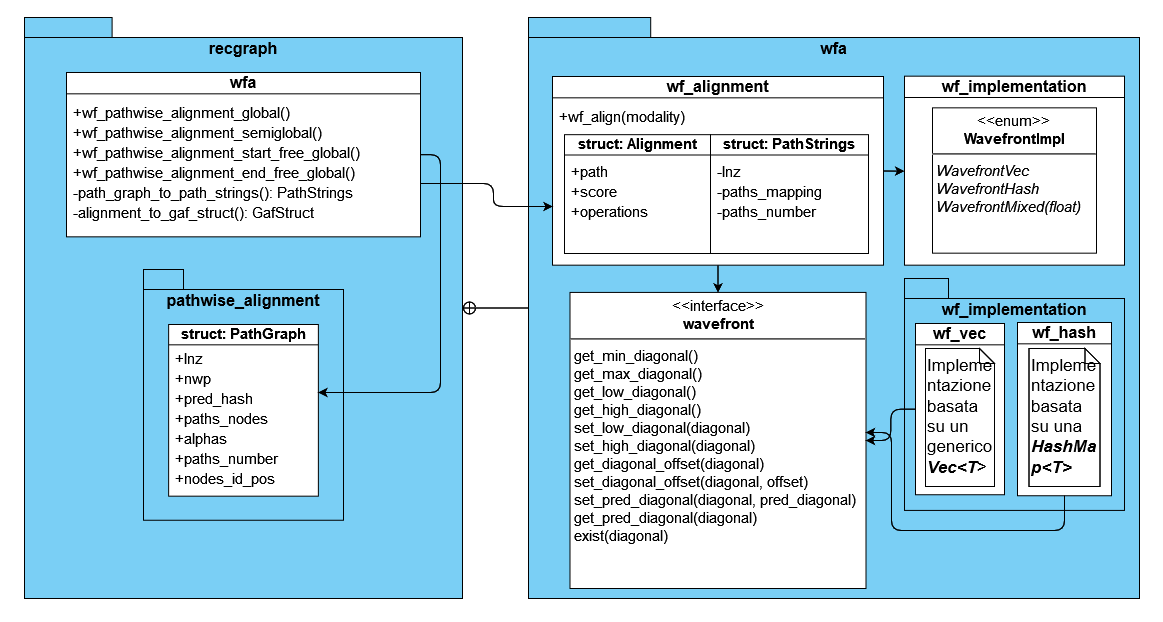
\includegraphics[width=1\linewidth]{images/wf_modules.png}
        \caption[Organizzazione modulare del prototipo]{\emph{Organizzazione modulare} del prototipo.}
        \label{fig:wf_modules}
    \end{figure}

    Come è possibile vedere dalla figura \ref{fig:wf_modules}, viene definita un'interfaccia \textbf{\textit{wfa}} che espone le quattro modalità di allineamento implementate:
    \begin{itemize}
        \item \textbf{\textit{wf\_pathwise\_alignment\_global}}, performa un allineamento in \emph{modalità globale};
        \item \textbf{\textit{wf\_pathwise\_alignment\_semiglobal}}, performa un allineamento in \emph{modalità semiglobale};
        \item \textbf{\textit{wf\_pathwise\_alignment\_start\_free\_global}}, performa un allineamento che può iniziare da qualsiasi vertice del grafo, ma vincolato a finire necessariamente nell'ultimo nodo;
        \item \textbf{\textit{wf\_pathwise\_alignment\_end\_free\_global}}, performa un allineamento che può finire in qualsiasi vertice del grafo, ma vincolato a iniziare necessariamente nel primo nodo.
    \end{itemize}
    Inoltre, all'interno del modulo sono contenute altre funzioni per convertire le \emph{strutture dati} utilizzate da \textbf{\textit{RecGraph}} in quelle utilizzate all'interno del package \textbf{\textit{wfa}}, contenente le seguenti componenti:
    \begin{itemize}
        \item \textbf{\textit{wavefront}}: interfaccia per definire le operazioni che deve implementare una struttura volta a rappresentare un \emph{fronte d'onda};
        \item \textbf{\textit{wf\_implementation}}: modulo che contiene le implementazioni disponibili per rappresentare un \emph{fronte d'onda} (devono implementare l'interfaccia \textbf{\textit{wavefront}});
        \item \textbf{\textit{wf\_alignment}}: modulo contenente le funzioni e le strutture dati che effettuano l'allineamento utilizzando l'algoritmo \textbf{\textit{wavefront}}.
    \end{itemize}
\subsection{Integrazione in RecGraph}
    Per integrare il protopipo all'interno di \textbf{\textit{RecGraph}} (al fine di utilizzare le già implementate funzionalità di lettura e scrittura di grafi) si è utilizzato il modulo \textbf{\textit{wfa}}, utilizzando direttamente le funzioni di allineamento esposte al posto di quelle di \textbf{\textit{RecGraph}}; lo stesso modulo si occupa della conversione delle differenti strutture dati utilizzate. La figura \ref{fig:wf_integration} mostra la \emph{struttura modulare} di \textbf{\textit{RecGraph}} e come è stato integrato il prototipo al suo interno.
        
    \begin{figure}[H]
        \centering
        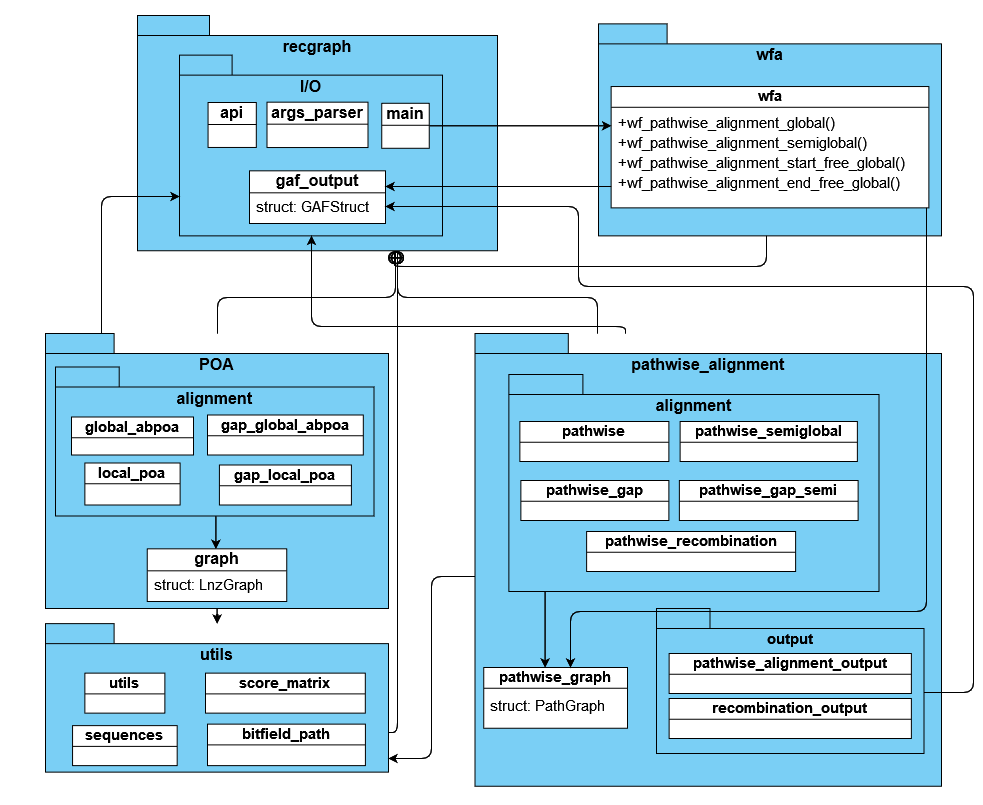
\includegraphics[width=1\linewidth]{images/wf_integration.png} 
        \caption[Integrazione]{Integrazione del prototipo in \textbf{\textit{RecGraph}}.}
        \label{fig:wf_integration}
    \end{figure}
    \vspace{20pt}
    \noindent
    Come è possibile vedere dalle \emph{relazioni di dipendenza}, il prototipo si serve soltanto delle due strutture dati \textbf{\textit{pathwise\_graph}} e \textbf{\textit{gaf\_output}}, utilizzate rispettivamente per rappresentare un \emph{grafo di variazione} e per contenere le informazioni di un allineamento in formato \emph{gaf}; inoltre, esso viene utilizzato direttamente all'interno del \textbf{\textit{main}}. Si riesce così a ottenere un basso accoppiamento dei moduli, pratica consigliata da \emph{design pattern} come \emph{low coupling}, al fine di diminuire l'impatto di eventuali futuri cambiamenti sul sistema.  

\section{Implementazione}
    In questa sezione si discutono le \textbf{scelte implementative} prese nella costruzione del prototipo, sviluppato tramite il linguaggio di programmazione \href{https://www.rust-lang.org/it}{\textbf{\textit{Rust}}.} 

\subsection{Interfaccia \textit{wavefront}}
    Modulo che definisce il \emph{trait} \textbf{\textit{Wavefront}} (struttura utilizzata in \textbf{\textit{Rust}} per definire un'\emph{interfaccia}), il quale specifica le operazioni che devono essere implementate per rappresentare un \emph{fronte d'onda}; per mantenere la complessità in tempo dell'algoritmo \emph{wavefront}, tutte le operazioni devono eseguite in $O(1)$. 
    
\subsection{Modulo \textit{wf\_implementation}}
    Modulo che definisce le implementazioni disponibili per rappresentare un \emph{fronte d'onda}: le definizioni si trova all'interno della \emph{enum} \textbf{\textit{WavefrontImpl}}, mentre le effettive implementazioni nel \emph{sotto-package} \textbf{\textit{wf\_implementation}} (figura \ref{fig:wf_modules}). In particolare, sono state fornite due implementazioni:
    \begin{itemize}
        \item \textbf{\textit{wf\_vec}}, memorizza il valore degli offsets delle diagonali all'interno di un \textbf{\textit{Vec}}; risulta \emph{più veloce} dell'altra implementazione, ma necessità di salvare anche gli offset delle diagonali che non vengono computate, generando uno \emph{spreco di memoria} e portando la \textbf{complessità in spazio} a 
        \begin{equation}
            T(n, m, p, \overline{d}) = O((n+m) \cdot \overline{d} \cdot p)
            \label{equation:space_complexity_wf_vec}
        \end{equation}
        \item \textbf{\textit{wf\_hash}}, salva il valore degli offsets delle diagonali all'interno di una \textbf{\textit{HashMap}}; può risultare particolarmente \emph{efficiente in memoria} quando il numero delle diagonali effettivamente computate è molto inferiore al totale, permettendo di evitare la memorizzazione di tutte le diagonali che non vengono computate e mantenendo l'\emph{andamento in memoria} a 
        \begin{equation}
            T(n, m, p, \overline{d}) = O(\overline{d}^2 \cdot p)
            \label{equation:space_complexity_wf_hash}
        \end{equation}
    \end{itemize}
    E' stata definita anche una terza implementazione, \textbf{\textit{WavefrontMixed}}, che cerca di unire i \emph{punti di forza} delle altre due: finchè la \emph{percentuale delle diagonali} che si sta computando è minore a una certa \textit{soglia parametrizzata}, viene scelto l'approccio \textbf{\textit{WavefrontHash}}, risparmiando così \emph{memoria} senza perdere troppo in \emph{tempo} (scegliendo soglie abbastanza basse, le diagonali effettivamente computate risultano molto inferiori a quelle totali, e la maggior parte del tempo dell'allineamento è richiesto quando il numero di diagonali che si stanno trattando cresce); superata la soglia, si passa invece all'implementazione \textbf{\textit{WavefrontVec}}, di cui viene ridotto lo \emph{spreco di memoria} (siccome il numero di diagonali che si stanno computando è vicino al massimo) e che risulta \emph{più veloce}.  
    
    Inoltre, il \emph{tipo degli interi} con cui vengono salvati gli offset risulta \emph{generico} sia in \textbf{\textit{wf\_vec}} che in \textbf{\textit{wf\_hash}}: a seconda delle dimensioni del \emph{grafo} e delle \emph{reads} in ingresso viene scelto in automatico il tipo più piccolo tra quelli disponibili (\textbf{\textit{u8}}, \textbf{\textit{u16}}, \textbf{\textit{u32}}, \textbf{\textit{u64}} e \textbf{\textit{u128}}), permettendo un significativo \emph{risparmio di memoria} (si osservi che per grafi con fino a 65535 nodi è possibile utilizzare degli \textbf{\textit{u16}}). 

\subsection{Modulo \textit{wf\_alignment}}
\label{section:wf_alignment}
    Modulo che si occupa di effettuare effettivamente l'allineamento tra il \emph{grafo di variazione} e la \emph{sequenza}. Nella figura \ref{fig:wf_alignment} viene fornito un diagramma che illustra le sue componenti più importanti:
    \begin{figure}[h]
        \centering
        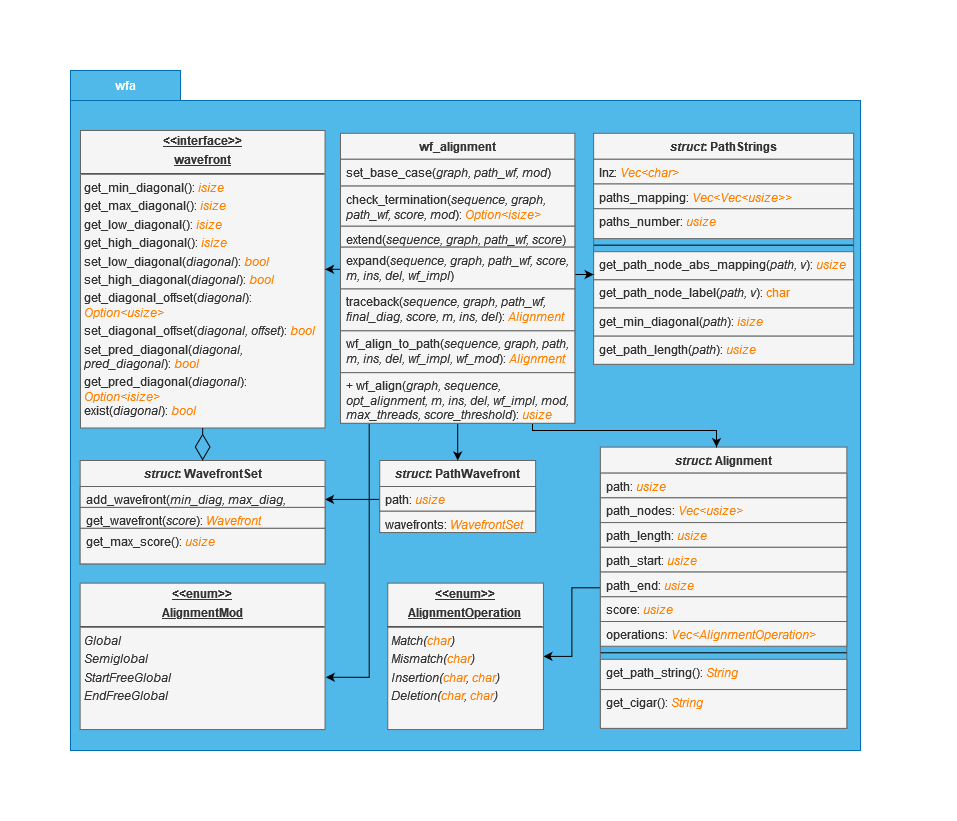
\includegraphics[width=1\linewidth]{images/wf_alignment_diagram.png} 
        \caption[Modulo allineamento]{Modulo \emph{wf\_alignment} per la gestione dell'allineamento.}
        \label{fig:wf_alignment}
        \end{figure}
    \clearpage

    In ingresso, il \emph{grafo di variazione} viene memorizzato tramite la \textbf{\textit{struct PathStrings}}, che essenzialmente estrae tutti i cammini del grafo; in output, invece, viene restituita un'istanza della \textbf{\textit{struct Alignment}}, contenente tutte le informazioni dell'allineamento effettuato.
    L'insieme dei \emph{fronti d'onda} computati per ogni \emph{punteggio} viene memorizzato nella \textbf{\textit{struct WavefrontSet}}: questa, insieme al \emph{cammino} che si sta trattando, va a comporre la \textbf{\textit{struct PathWavefront}}, che contiene tutte le informazioni necessarie per effettuare l'allineamento a un percorso.
    A livello di interfaccia viene esposta solamente una funzione, \textbf{\textit{wf\_align}}, che si occupa di gestire gli allineamenti tra i percorsi del grafo, lanciando un \emph{thread} per ogni percorso e selezionando il miglior allineamento trovato. In particolare, riceve in ingresso\footnote{Per ragioni di leggibilità, sono stati riportati solo i parametri più importanti.}
    \begin{itemize}
        \item \emph{il grafo di variazione} (come \textbf{\textit{PathStrings}}),
        \item la \emph{sequenza} da allineare,
        \item un \emph{array} dove inserire gli allineamenti ottimali trovati (come \textbf{\textit{Alignment}}),
        \item le \emph{penalità} di \textbf{\textit{mismatch}}, \textbf{\textit{inserimento}} e \textbf{\textit{cancellazione}}.
        \item la \emph{modalità di allineamento} (una voce della \emph{enum} \textbf{\textit{AlignmentMod}}),
        \item il numero massimo di \emph{thread} da eseguire in parallelo,
        \item una \emph{soglia} a cui troncare l'allineamento (facoltativa)
    \end{itemize}
    e restituisce il valore dell'allineamento prodotto. Inoltre, ogni volta che un thread termina un allineamento, viene impostata (o eventualmente aggiornata) una \emph{soglia} sul \emph{massimo punteggio raggiungibile}, condivisa da tutti i thread: ogni allineamento che supera tale soglia viene abbandonato. 
    Ogni thread lanciato esegue la funzione \textbf{\textit{wf\_align\_to\_path}}, che esegue l'algoritmo \emph{wavefront} tra un percorso del grafo e una sequenza (quindi tra due stringhe), alternando le già discusse fasi di \emph{estensione} ed \emph{espansione}.
\clearpage

\section{Benchmark}
    In seguito vengono riportate alcune sperimentazioni eseguite per osservare il comportamento del prototipo. In particolare, nella prima sezione si analizzano le performance dell'\emph{allineamento} \textbf{\textit{wavefront}} rispetto a \textbf{\textit{RecGraph}}, mentre nella sezione successiva si tratta l'andamento delle prestazioni del prototipo rispetto a diversi \textbf{gradi di libertà} (\emph{punteggio dell'allineamento}, \emph{numero di thread utilizzati}, \emph{numero di cammini del grafo di variazione}). La sperimentazione è stata eseguita su un server con 64 core e 256 GB di RAM. Per quanto riguarda le grandezze in input, si fa riferimento alla seguente notazione:
    \begin{itemize}
        \item \textbf{\textit{n}}: lunghezza media dei cammini del \emph{grafo di variazione};
        \item \textbf{\textit{p}}: numero di cammini del \emph{grafo di variazione};
        \item \textbf{\textit{m}}: lunghezza della \emph{sequenza};
        \item \textbf{\textit{d}}: valore ottimale dell'allineamento. 
    \end{itemize}

\subsection{RecGraph vs Wavefront}
\subsubsection{Grafo di variazione}
    In questa prima fase della sperimentazione è stato usato il \textbf{grafo di variazione} descritto nella tabella \ref{tab:graph}:
    \vspace{20pt}
    \begin{table}[ht]
        \centering
        \begin{tabular}{|c|c|c|c|}
        \hline
        \multicolumn{4}{|c|}{\multirow{2}{*}{\textbf{Variation graph}}} \\
        \multicolumn{4}{|c|}{} \\
        \hline
        \textbf{Linearization} & \multicolumn{3}{|c|}{\textbf{Paths}} \\
        \hline
        \textbf{Length (bp)} & \textbf{Number} & \textbf{Paths mean length (bp)} & \textbf{Paths for node} \\
        \hline
        49376 & 30 & 29744 & 18.1 (60\%) \\
        \hline
        \end{tabular}
        \caption{Caratteristiche del \emph{grafo di variazione} usato nel benchmark.}
        \label{tab:graph}
    \end{table}
    \vspace{10pt}
    
    In questa istanza si nota un'importante \emph{sovrapposizione dei cammini}: per ogni nodo, infatti, passano in media 18 cammini su 30 totali (più del 60\%). Questa caratteristica va a penalizzare l'implementazione dell'algoritmo \textbf{\textit{wavefront}} in quanto, basandosi sull'estrazione dei cammini dal grafo per permettere il \textbf{\textit{multithreading}}, va a computare diverse volte i valori degli allineamenti per gli stessi nodi condivisi da più percorsi; al contrario, \textbf{\textit{RecGraph}} sfrutta a suo vantaggio questa proprietà, memorizzando soltanto il punteggio di un solo percorso per i nodi condivisi (ottimizzazione del \textbf{\textit{reference path}} (sezione \ref{section:recgraph})).   

    \vspace{20pt}
    Si riportano i risultati ottenuti su \textbf{reads} di diversa lunghezza, sia in \textbf{modalità globale} che in \textbf{modalità semiglobale}.

\subsubsection{Modalità globale}
    Per la sperimentazione in \textbf{modalità globale} sono state usate \emph{sequenze} di lunghezza 150 bp, 1000 bp, 10000 bp e 25000 bp; i seguenti valori rigurdano allineamenti eseguiti utilizzando \textbf{\textit{RecGraph}}:
    \vspace{20pt}
    \begin{table}[h]
        \centering
        \begin{tabular}{|c|c|c|c|c|c|c|c|}
        \hline
        \multicolumn{8}{|c|}{\multirow{2}{*}{\textbf{Modality:} \emph{Global}}} \\
        \multicolumn{8}{|c|}{} \\
        \hline
        & \multicolumn{2}{|c|}{\textbf{Reads}} & \multicolumn{4}{|c|}{\textbf{Time (s)}} & \textbf{Memory (GB)} \\
        \hline
        \textbf{Algorithm} & \textbf{N} & \textbf{L} & \textbf{Tot} & \textbf{Mean} & \textbf{Max} & \textbf{Min} & \textbf{Max} \\
        \hline
        \multirow{4}{*}{\emph{RecGraph}} & 25 & 150 & 75 & 3.0 & 3.6 & 2.5 & 2.17 \\
        \cline{2-8}
        & \multirow{2}{*}{10} & 1000 & \multirow{2}{*}{214} & 21.4 & 26.4 & 20.0 & 7.84 \\
        & & $6.7 \times$ & & $7.1 \times$ & $7.3 \times$ & $8 \times$ & $3.6 \times$ \\
        \cline{2-8}
        & \multirow{2}{*}{5} & 10000 & \multirow{2}{*}{1155} & 231.1 & 241.4 & 216.2 & 75.64 \\
        & & $66.7 \times$ & & $77.0 \times$ & $67.1 \times$ & $86.5 \times$ & $34.8 \times$ \\
        \cline{2-8}
        & \multirow{2}{*}{5} & 25000 & \multirow{2}{*}{6909} & 690.9 & 703.2 & 678.5 & 192.45 \\
        & & $167 \times$ & & $230 \times$ & $195 \times$ & $271.4 \times$ & $88.7 \times$ \\
        \hline
        \end{tabular}
        \caption{Benchmark per \textbf{\textit{RecGraph}} in \emph{modalità globale}.}
        \label{tab:benchmark_RecGraph_global}
    \end{table}
    \vspace{10pt}
    
   I dati evidenziano una \textbf{complessità lineare} nella \textit{lunghezza delle sequenze}, sia per quanto riguarda il \textbf{tempo} che per lo \textbf{spazio}, in linea con la complessità $O(n \cdot m \cdot p)$ attesa. Sulle \textbf{reads} di lunghezza $25000$ bp inizia a essere necessaria anche un'importante quantità di memoria ($\approx$ 200 GB).
   
   \vspace{20pt} 
    A seguire invece i valori ottenuti dall'algoritmo \textbf{\textit{wavefront}} con \emph{distanza di edit unitaria}:
    \vspace{20pt}
    \begin{table}[h]
        \centering
        \begin{tabular}{|c|c|c|c|c|c|c|c|c|}
        \hline
        \multicolumn{9}{|c|}{\multirow{2}{*}{\textbf{Modality:} \emph{Global}}} \\
        \multicolumn{9}{|c|}{} \\
        \hline
        & \multicolumn{2}{|c|}{\textbf{Reads}} & \multicolumn{4}{|c|}{\textbf{Time (s)}} & \textbf{Memory (GB)} & \textbf{Score} \\
        \hline
        \textbf{Algorithm} & \textbf{N} & \textbf{L} & \textbf{Tot} & \textbf{Mean} & \textbf{Max} & \textbf{Min} & \textbf{Max} & \textbf{Mean} \\
        \hline
        \multirow{4}{*}{\emph{wf\_edit-distance}} & 25 & 150 & 545 & 21.8 & 24.5 & 20.2 & 111.33 & 28879 \\
        \cline{2-9}
        & \multirow{2}{*}{10} & 1000 & \multirow{2}{*}{222} & 22.2 & 24.9 & 20.2 & 110.32 & 28029 \\
        & & $6.7 \times$ & & $1.02 \times$ & $1.02 \times$ & $1 \times$ & $0.99 \times$ & $0.97 \times$\\
        \cline{2-9}
        & \multirow{2}{*}{5} & 10000 & \multirow{2}{*}{139.7} & 28.0 & 29.0 & 26.8 & 111.23 & 19669 \\
        & & $66.7 \times$ & & $1.28 \times$ & $1.18 \times$ & $1.34 \times$ & $1.0 \times$ & $0.68 \times$\\
        \cline{2-9}
        & \multirow{2}{*}{5} & 25000 & \multirow{2}{*}{134} & 13.4 & 15.1 & 12.1 & 64.42 & 8149\\
        & & $167 \times$ & & $0.6 \times$ & $0.6 \times$ & $0.6 \times$ & $0.58 \times$ & $0.28 \times$ \\
        \hline
        \end{tabular}
        \caption{Benchmark per \textbf{\textit{wf\_edit-distance}} in \emph{modalità globale}.}
        \label{tab:benchmark_wf_edit-dist_global}
    \end{table}
    \vspace{10pt}

    Qui si nota un andamento del tutto diverso: l'allineamento risulta \emph{meno performante} per le sequenze di lunghezza 150 bp, 1000 bp e 10000 bp (che producono punteggi di allineamento molto alti), mentre risulta più \emph{efficiente} per le sequenze di 25000 bp, migliorando sia in \textbf{tempo di esecuzione} sia in \textbf{memoria occupata} in accordo con la complessità $O(\min\{n, m\} \cdot \overline{d} \cdot p)$ prevista. 

    Di seguito un confronto dei valori ottenuti dalle esecuzioni di \textbf{\textit{RecGraph}} e di \textbf{\textit{wf\_edit-distance}} per sequenze della stessa lunghezza:

\vspace{20pt}
    \begin{table}[h]
        \centering
        \begin{tabular}{|c|c|c|c|c|c|}
            \hline
                \multicolumn{2}{|c|}{\textbf{Modality:} \emph{Global}} & \multicolumn{2}{|c|}{\textbf{Reads number: } \emph{25}} & \multicolumn{2}{|c|}{\textbf{Reads length:} \emph{150 bp}} \\
            \hline
                \multicolumn{6}{|c|}{} \\
            \hline
                & \multicolumn{4}{|c|}{\textbf{Time (s)}} & \textbf{Memory (GB)} \\
            \hline
                \textbf{Algorithm} & \textbf{Tot} & \textbf{Mean} & \textbf{Max} & \textbf{Min} & \textbf{Max} \\
            \hline
                \emph{RecGraph} & 75 & 3.0 & 3.6 & 2.5 & 2.17 \\
            \hline
                \multirow{2}{*}{\emph{wf\_edit-distance}} & 545 & 21.4 & 24.5 & 20.2 & 111.33 \\
                & $7.3 \times$ & $7.3 \times$ & $7.5 \times$ & $9 \times$ & $51 \times$ \\
            \hline
            \multirow{2}{*}{\emph{wf\_weighted\_edit-distance}} & 1097 & 43.9 & 47.1 & 43.0 & 223.59 \\
                & $14.6 \times$ & $14.6 \times$ & $13.1 \times$ & $17.2 \times$ & $103 \times$ \\
            \hline
        \end{tabular}
        \caption{Benchmark per \emph{reads} di 150 bp in \emph{modalità globale}. Nella modalità \textbf{\textit{wf\_weighted-edit-distance}}, sono state usate le seguenti penalità: \textbf{mismatch=1}, \textbf{insertion=2}, \textbf{deletion=2}.}
        \label{tab:benchmark_global_150}
    \end{table}
    \vspace{20pt}
    
    \begin{table}[h]
        \centering
        \begin{tabular}{|c|c|c|c|c|c|}
            \hline
                \multicolumn{2}{|c|}{\textbf{Modality:} \emph{Global}} & \multicolumn{2}{|c|}{\textbf{Reads number: }   \emph{10}} & \multicolumn{2}{|c|}{\textbf{Reads length:} \emph{1000 bp}} \\
            \hline
                \multicolumn{6}{|c|}{} \\
            \hline
                & \multicolumn{4}{|c|}{\textbf{Time (s)}} & \textbf{Memory (GB)} \\
            \hline
                \textbf{Algorithm} & \textbf{Tot} & \textbf{Mean} & \textbf{Max} & \textbf{Min} & \textbf{Max} \\
            \hline
                \emph{RecGraph} & 214 & 21.4 & 26.4 & 20.0 & 7.84 \\
            \hline
                \multirow{2}{*}{\emph{wf\_edit-distance}} & 222 & 22.2 & 24.9 & 20.2 & 110.32 \\
                & $1.04 \times$ & $1.04 \times$ & $0.94 \times$ & $1 \times$ & $14 \times$ \\
            \hline
            \multirow{2}{*}{\emph{wf\_weighted\_edit-distance}} & 464.0 & 46.4 & 46.9 & 46.0 & 223.61 \\
                & $2.2 \times$ & $2.2  \times$ & $1.78 \times$ & $2.3 \times$ & $28.5 \times$ \\
            \hline
        \end{tabular}
        \caption{Benchmark per \emph{reads} di 1000 bp in \emph{modalità globale}. Nella modalità \textbf{\textit{wf\_weighted-edit-distance}}, sono state usate le seguenti penalità: \textbf{mismatch=1}, \textbf{insertion=2}, \textbf{deletion=2}.}
        \label{tab:benchmark_global_1k}
    \end{table}
    \vspace{20pt}
    
    \begin{table}[h]
        \centering
        \begin{tabular}{|c|c|c|c|c|c|}
            \hline
                \multicolumn{2}{|c|}{\textbf{Modality:} \emph{Global}} & \multicolumn{2}{|c|}{\textbf{Reads number: } \emph{5}} & \multicolumn{2}{|c|}{\textbf{Reads length:} \emph{10000 bp}} \\
            \hline
                \multicolumn{6}{|c|}{} \\
            \hline
                & \multicolumn{4}{|c|}{\textbf{Time (s)}} & \textbf{Memory (GB)} \\
            \hline
                \textbf{Algorithm} & \textbf{Tot} & \textbf{Mean} & \textbf{Max} & \textbf{Min} & \textbf{Max} \\
            \hline
                \emph{RecGraph} & 1155 & 231.1 & 241.4 & 216.2 & 75.64 \\
            \hline
                \multirow{2}{*}{\emph{wf\_edit-distance}} & 139.7 & 28.0 & 29.0 & 26.8 & 111.23 \\
                & $0.12 \times$ & $0.12  \times$ & $0.12 \times$ & $0.12 \times$ & $1.47 \times$ \\
            \hline
            \multirow{2}{*}{\emph{wf\_weighted\_edit-distance}} & 287.0 & 57.3 & 56.4 & 59.6 & 196.73 \\
                & $0.25 \times$ & $0.25  \times$ & $0.23 \times$ & $0.28 \times$ & $2.6 \times$ \\
            \hline
        \end{tabular}
        \caption{Benchmark per \emph{reads} di 10000 bp in \emph{modalità globale}. Nella modalità \textbf{\textit{wf\_weighted-edit-distance}}, sono state usate le seguenti penalità: \textbf{mismatch=1}, \textbf{insertion=2}, \textbf{deletion=2}.}
        \label{tab:benchmark_global_10k}
    \end{table}
    \vspace{20pt}
\clearpage
    
    \begin{table}[h]
        \centering
        \begin{tabular}{|c|c|c|c|c|c|}
            \hline
                \multicolumn{2}{|c|}{\textbf{Modality:} \emph{Global}} & \multicolumn{2}{|c|}{\textbf{Reads number: } \emph{5}} & \multicolumn{2}{|c|}{\textbf{Reads length:} \emph{25000 bp}} \\
            \hline
                \multicolumn{6}{|c|}{} \\
            \hline
                & \multicolumn{4}{|c|}{\textbf{Time (s)}} & \textbf{Memory (GB)} \\
            \hline
                \textbf{Algorithm} & \textbf{Tot} & \textbf{Mean} & \textbf{Max} & \textbf{Min} & \textbf{Max} \\
            \hline
                \emph{RecGraph} & 6909 & 690.9 & 703.2 & 678.5 & 192.45 \\
            \hline
                \multirow{2}{*}{\emph{wf\_edit-distance}} & 134.0 & 13.4 & 15.1 & 12.1 & 64.42 \\
                & $0.02 \times$ & $0.02  \times$ & $0.02 \times$ & $0.02 \times$ & $0.33 \times$ \\
            \hline
                \multirow{2}{*}{\emph{wf\_weighted\_edit-distance}} & 190.0 & 19.0 & 20.9 & 17.7 & 95.16 \\
                & $0.03 \times$ & $0.03  \times$ & $0.03 \times$ & $0.03 \times$ & $0.49 \times$ \\
            \hline
        \end{tabular}
        \caption{Benchmark per \emph{reads} di 25000 bp in \emph{modalità globale}. Nella modalità \textbf{\textit{wf\_weighted-edit-distance}}, sono state usate le seguenti penalità: \textbf{mismatch=1}, \textbf{insertion=2}, \textbf{deletion=2}.}
        \label{tab:benchmark_global_25k}
    \end{table}
    \vspace{20pt}
    
    e una \textbf{visualizzazione grafica} dei dati precedentemente riportati (figura \ref{fig:global_comparison}):
    \begin{figure}[!h]
        \centering
        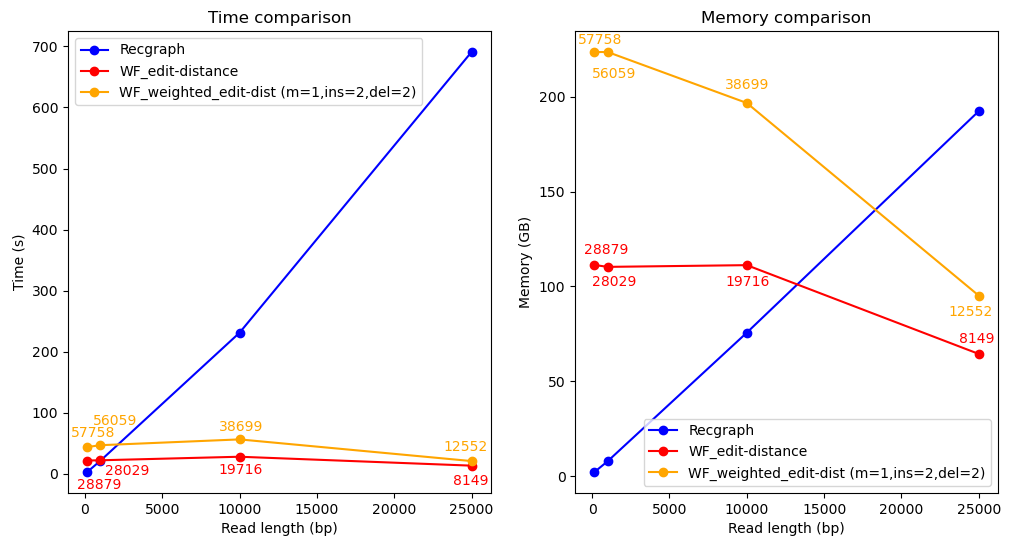
\includegraphics[width=1.0\linewidth]{images/global_comparison.png} 
        \caption[Confronto modalità globale]{Confronto in termini di tempo e spazio per l'allineamento in \textbf{modalità globale} tra \emph{RecGraph} e \emph{wf\_alignment\_edit-distance}. I numeri riportati rappresentano le \textbf{distanze di edit} computate da \emph{wf\_alignment\_edit-distance}.}
        \label{fig:global_comparison}
    \end{figure}
    \vspace{20pt}
    
    Nella \emph{modalità globale}, risulta poco sensato l'utilizzo di \textbf{\textit{wf\_edit-distance}} quando le sequenze sono molto \emph{più corte} dei cammini del grafo; al contrario, diventa estremamente interessante il suo impiego (sia in termini di \textbf{tempo di esecuzione} che di \textbf{memoria occupata}) quando la \emph{dimensione delle reads} diventa \emph{paragonabile} a quella dei \emph{cammini}, usando eventualmente anche \emph{penalità non unitarie}. 
    \clearpage
    
\subsubsection{Modalità semiglobale}
    Si riportano ora i risultati ottenuti ottenuti in \textbf{modalità semiglobale}, per la quale sono state usate \emph{reads} di lunghezza 150 bp, 1000 bp e 10000 bp; si mostrano per primi nuovamente i valori ottenuti utilizzando \textbf{\textit{RecGraph}}:
    \vspace{20pt}
    \begin{table}[h]
        \centering
        \begin{tabular}{|c|c|c|c|c|c|c|c|}
            \hline
                \multicolumn{8}{|c|}{\multirow{2}{*}{\textbf{Modality:} \emph{Semiglobal}}} \\
                \multicolumn{8}{|c|}{} \\
            \hline
                & \multicolumn{2}{|c|}{\textbf{Reads}} & \multicolumn{4}{|c|}{\textbf{Time (s)}} & \textbf{Memory (GB)} \\
            \hline
                \textbf{Algorithm} & \textbf{N} & \textbf{L} & \textbf{Tot} & \textbf{Mean} & \textbf{Max} &  \textbf{Min} & \textbf{Max} \\
            \hline
                \multirow{4}{*}{\emph{RecGraph}} & 100 & 150 & 270 & 2.7 & 3.1 & 2.3 & 2.67 \\
            \cline{2-8}
                & \multirow{2}{*}{25} & 1000 & \multirow{2}{*}{483} & 19.3 & 22.3 & 18.5 & 7.84 \\
                & & $6.7 \times$ & & $4.6 \times$ & $7.2 \times$ & $8 \times$ & $2.9 \times$ \\
            \cline{2-8}
                & \multirow{2}{*}{5} & 10000 & \multirow{2}{*}{1080} & 216 & 223 & 208.1 & 75.66 \\
                & & $66.7 \times$ & & $80 \times$ & $71.9 \times$ & $90.5 \times$ & $28.3 \times$ \\
            \hline
        \end{tabular}
        \caption{Benchmark per \emph{RecGraph} in \emph{modalità semiglobale}.}
        \label{tab:benchmark_RecGraph_semiglobal}
    \end{table}
    \vspace{20pt}
    
    Come da previsione, i risultati ottenuti sono molto simili a quelli della \textbf{modalità globale} (tabella \ref{tab:benchmark_RecGraph_global}): infatti, in entrambe le modalità, \textbf{\textit{RecGraph}} computa allo stesso modo l'intera \emph{matrice di programmazione dinamica}, mantenendo quindi la stessa \emph{complessità}: le differenze stanno nelle diverse \emph{condizioni iniziali} e nella selezione della \emph{soluzione ottimale}.
    
    Al contrario, i risultati ottenuti da \textbf{\textit{wf\_edit\_distance}} cambiano radicalmente:
    \vspace{20pt}
    \begin{table}[h]
        \centering
        \begin{tabular}{|c|c|c|c|c|c|c|c|c|}
            \hline
                \multicolumn{9}{|c|}{\multirow{2}{*}{\textbf{Modality:} \emph{Semiglobal}}} \\
                \multicolumn{9}{|c|}{} \\
            \hline
                & \multicolumn{2}{|c|}{\textbf{Reads}} & \multicolumn{4}{|c|}{\textbf{Time (s)}} & \textbf{Memory (GB)} & \textbf{Score} \\
            \hline
                \textbf{Algorithm} & \textbf{N} & \textbf{L} & \textbf{Tot} & \textbf{Mean} & \textbf{Max} & \textbf{Min} & \textbf{Max} & \textbf{Mean} \\
            \hline
                \multirow{4}{*}{\emph{wf\_edit-dist}} & 100 & 150 & 2.02 & 0.02 & 0.2 & 0.01 & 0.138 & $<5$ \\
            \cline{2-9}
                & \multirow{2}{*}{25} & 1000 & \multirow{2}{*}{2.869} & 0.1 & 0.3 & 0.1 & 0.212 & 22.5 \\
                & & $6.7 \times$ & & $5 \times$ & $1.5 \times$ & $10.0 \times$ & $1.34 \times$ & $1.5 \times$ \\
            \cline{2-9}
                & \multirow{2}{*}{5} & 10000 & \multirow{2}{*}{18.4} & 3.7 & 4.4 & 3.2 & 5.07 & 1051 \\
                & & $66.7 \times$ & & $185 \times$ & $22.0 \times$ & $320 \times$ & $36.7 \times$ & $260 \times$\\
            \hline
        \end{tabular}
        \caption{Benchmark per \emph{wf\_edit-distance} in \emph{modalità semiglobale}.}
        \label{tab:benchmark_wf_edit-dist_semiglobal}
    \end{table}
    \vspace{20pt}

    L'\textbf{allineamento semiglobale} permette di allineare le sequenze a qualsiasi punto del grafo, ottenendo \textbf{distanze di edit} nettamente inferiori che aumentano in maniera proporzionale alla lunghezza delle reads. Come conseguenza, anche \textbf{\textit{wf\_edit-distance}} scala in maniera proporzionale alla lunghezza delle sequenze. 

    \vspace{20pt}
    Di seguito un confronto dei valori ottenuti da \textbf{\textit{RecGraph}} e da \textbf{\textit{wf\_edit\_distance}} (sia con penalità unitarie che nel caso pesato) sulle sequenze di interesse:

    \begin{table}[h]
        \centering
        \begin{tabular}{|c|c|c|c|c|c|}
            \hline
             \multicolumn{2}{|c|}{\textbf{Modality:} \emph{Semiglobal}} & \multicolumn{2}{|c|}{\textbf{Reads number: } \emph{100}} & \multicolumn{2}{|c|}{\textbf{Reads length:} \emph{150 bp}} \\
            \hline
                \multicolumn{6}{|c|}{} \\
            \hline
                & \multicolumn{4}{|c|}{\textbf{Time (s)}} & \textbf{Memory (GB)} \\
            \hline
                \textbf{Algorithm} & \textbf{Tot} & \textbf{Mean} & \textbf{Max} & \textbf{Min} & \textbf{Max} \\
            \hline
                \emph{RecGraph} & 270 & 2.7 & 3.1 & 2.3 & 2.67 \\
            \hline
                \multirow{2}{*}{\emph{wf\_edit-distance}} & 2.02 & 0.02 & 0.2 & 0.01 & 0.138 \\
                & $<0.01 \times$ & $<0.01 \times$ & $0.06 \times$ & $<0.01 \times$ & $0.05 \times$ \\
            \hline
                \multirow{2}{*}{\emph{wf\_weighted\_ed}} & 3.27 & 0.024 & 0.2 & 0.01 & 0.165 \\
                & $0.01 \times$ & $0.01 \times$ & $0.06 \times$ & $<0.01 \times$ & $0.06 \times$ \\
            \hline
        \end{tabular}
        \caption{Benchmark per \emph{reads} di 150 bp in \emph{modalità semiglobale}. Nella modalità \textbf{\textit{wf\_weighted-edit-distance}}, sono state usate le seguenti penalità: \textbf{mismatch=1}, \textbf{insertion=2}, \textbf{deletion=2}.}
        \label{tab:benchmark_semiglobal_150}
    \end{table}
    \vspace{20pt}
    
    \begin{table}[h]
        \centering
        \begin{tabular}{|c|c|c|c|c|c|}
            \hline
                \multicolumn{2}{|c|}{\textbf{Modality:} \emph{Semiglobal}} & \multicolumn{2}{|c|}{\textbf{Reads number: } \emph{25}} & \multicolumn{2}{|c|}{\textbf{Reads length:} \emph{1000 bp}} \\
            \hline
                \multicolumn{6}{|c|}{} \\
            \hline
                & \multicolumn{4}{|c|}{\textbf{Time (s)}} & \textbf{Memory (GB)} \\
            \hline
                \textbf{Algorithm} & \textbf{Tot} & \textbf{Mean} & \textbf{Max} & \textbf{Min} & \textbf{Max} \\
            \hline
                \emph{RecGraph} & 483 & 19.3 & 22.3 & 18.5 & 7.84 \\
            \hline
                \multirow{2}{*}{\emph{wf\_edit-distance}} & 2.87 & 0.1 & 0.3 & 0.1 & 0.212 \\
                & $<0.01 \times$ & $<0.01 \times$ & $0.01 \times$ & $<0.01 \times$ & $0.03 \times$ \\
            \hline
                \multirow{2}{*}{\emph{wf\_weighted\_edit-distance}} & 3.22 & 0.1 & 0.4 & 0.1 & 0.351 \\
                & $<0.01 \times$ & $<0.01 \times$ & $0.02 \times$ & $<0.01 \times$ & $0.05 \times$ \\
            \hline
        \end{tabular}
        \caption{Benchmark per \emph{reads} di 1000 bp in \emph{modalità semiglobale}. Nella modalità \textbf{\textit{wf\_weighted-edit-distance}}, sono state usate le seguenti penalità: \textbf{mismatch=1}, \textbf{insertion=2}, \textbf{deletion=2}.}
        \label{tab:benchmark_semiglobal_1k}
    \end{table}
    \vspace{20pt}
    
    \begin{table}[h]
        \centering
        \begin{tabular}{|c|c|c|c|c|c|}
            \hline
                \multicolumn{2}{|c|}{\textbf{Modality:} \emph{Semiglobal}} & \multicolumn{2}{|c|}{\textbf{Reads number: } \emph{5}} & \multicolumn{2}{|c|}{\textbf{Reads length:} \emph{10000 bp}} \\
            \hline
                \multicolumn{6}{|c|}{} \\
            \hline
                & \multicolumn{4}{|c|}{\textbf{Time (s)}} & \textbf{Memory (GB)} \\
            \hline
                \textbf{Algorithm} & \textbf{Tot} & \textbf{Mean} & \textbf{Max} & \textbf{Min} & \textbf{Max} \\
            \hline
                \emph{RecGraph} & 1080 & 216 & 223 & 208.1 & 75.66 \\
            \hline
                \multirow{2}{*}{\emph{wf\_edit-distance}} & 18.4 & 3.7 & 4.4 & 3.2 & 5.07 \\
                & $0.02 \times$ & $0.02  \times$ & $0.02 \times$ & $0.02 \times$ & $0.08 \times$ \\
            \hline
                \multirow{2}{*}{\emph{wf\_weighted\_edit-distance}} & 18.8 & 3.8 & 4.3 & 3.4 & 5.68 \\
                & $0.02 \times$ & $0.02 \times$ & $0.02 \times$ & $0.02 \times$ & $0.08 \times$ \\
            \hline
        \end{tabular}
        \caption{Benchmark per \emph{reads} di 10000 bp in \emph{modalità semiglobale}. Nella modalità \textbf{\textit{wf\_weighted-edit-distance}}, sono state usate le seguenti penalità: \textbf{mismatch=1}, \textbf{insertion=2}, \textbf{deletion=2}.}
        \label{tab:benchmark_semiglobal_10k}
    \end{table}
    \vspace{20pt}
    
    e un \textbf{plotting} dei risultati appena riportati (figura \ref{fig:semiglobal_comparison}):
    \clearpage
    \begin{figure}[t]
        \centering
        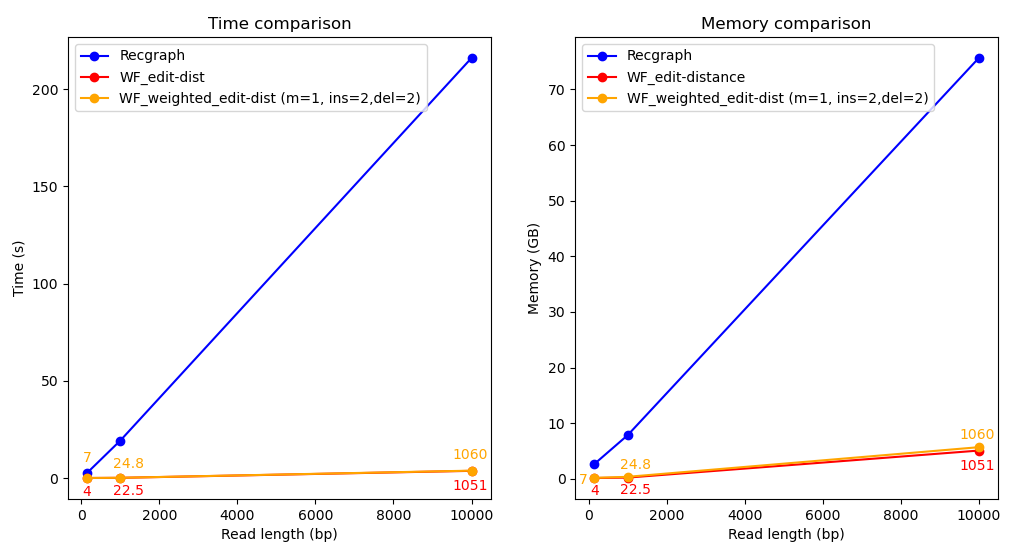
\includegraphics[width=1.0\linewidth]{images/semiglobal_comparison.png} 
        \caption[Confronto modalità semiglobale]{Confronto in termini di tempo e spazio per l'allineamento in \textbf{modalità semiglobale} tra \emph{RecGraph} e \emph{wf\_alignment\_edit-distance}. I numeri riportati rappresentano le \textbf{distanze di edit} computate da \emph{wf\_alignment\_edit-distance}.}
        \label{fig:semiglobal_comparison}
    \end{figure}
    
    Nella \textbf{modalità semiglobale}, \textbf{\textit{wf\_edit\_distance}} risulta superiore a \textbf{\textit{RecGraph}} su tutti gli input, sia in \textbf{tempo di esecuzione} che in \textbf{memoria}.
    
\subsection{Analisi dell'andamento del prototipo su singole variabili}

    In questa seconda parte del benchmark ci si è concentrati in maniera specifica sull'analisi dell'andamento asintotico di \textbf{\textit{wf\_edit\_distance}}: prese come riferimento $n$ variabili, si è andato a misurare l'andamento di ognuna di esse fissando la restanti $n-1$ come costanti. In particolare, si sono considerate le seguenti dimensioni:
    \begin{itemize}
        \item \emph{valore dell'allineamento};
        \item \emph{numero di threads} lanciati in parallelo;
        \item \emph{numero di cammini} del \emph{grafo di variazione}.
    \end{itemize}
    Si è utilizzato come input lo stesso grafo utilizzato in precedenza (tabella \ref{tab:graph}) e delle sequenze della stessa lunghezza dei suoi cammini, eseguendo allineamenti in \textbf{modalità globale}.
    
    Dove non specificato diversamente, il \textbf{cammino ottimale} è stato inserito a metà di tutti i percorsi; inoltre è stato utilizzato un \emph{singolo thread} (tranne ovviamente nella sperimentazione sul numero dei threads). Come implementazione del \emph{fronte d'onda} è stato scelto \textbf{\textit{wf\_vec}}. 
    
    Si ricorda che la \textbf{complessità temporale} attesa dell'algoritmo è
    \begin{equation}
        T(n, m, p, \overline{d}) = O(\min\{n, m\} \cdot \overline{d} \cdot p)
        \label{equation:wf_time_complexity_benchmark}
    \end{equation}
    mentre la \textbf{complessità in spazio} è
    \begin{equation}
        T(n, m, p, \overline{d}) = O((n+m) \cdot \overline{d} \cdot p)
        \label{equation:wf_space_complexity_benchmark}
    \end{equation}
    a causa dell'implementazione \textbf{\textit{wf\_vec}} scelta (equazione \ref{equation:space_complexity_wf_vec}).

    \vspace{20pt}
    A seguire i risultati ottenuti.

\subsubsection{Numero di threads variabile}
     \begin{figure}[h]
        \centering
        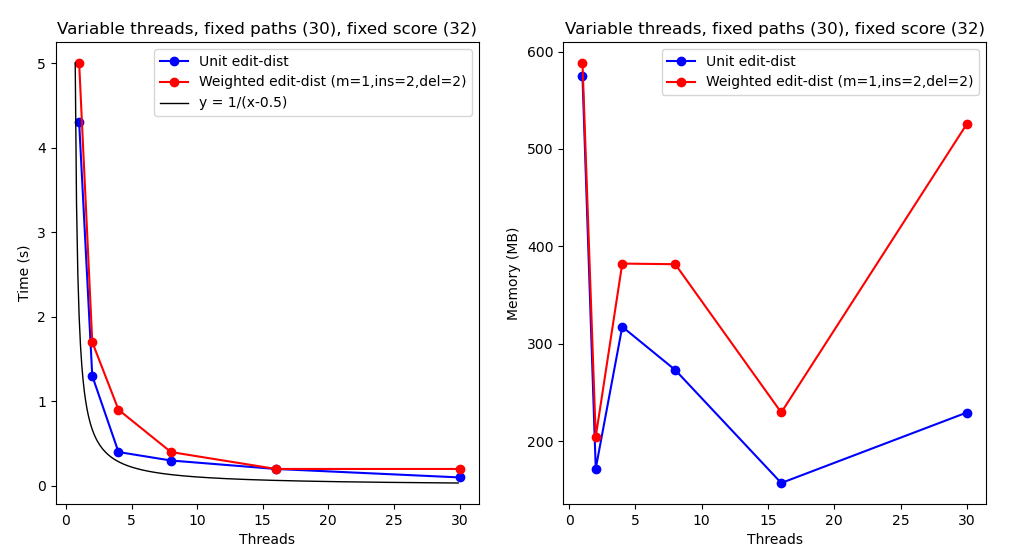
\includegraphics[width=1.0\linewidth]{images/benchmark_threads_variable.png} 
         \caption[Andamento con threads variabili]{Andamento in \emph{tempo} di \textbf{\textit{wf\_alignment}} rispetto a un \emph{numero di threads} eseguiti in parallelo \emph{variabile}.}
        \label{fig:benchmark_threads}
    \end{figure}
    \vspace{20pt}

    Facendo variare il \textbf{numero di threads} eseguiti in parallelo si evidenzia un \emph{andamento asintotico temporale} del tipo $y = \frac{1}{x}$, come da previsione. L'andamento in \emph{memoria} risulta molto più imprevedibile, anche in questo caso come conseguenza del troncamento rispetto all' allineamento migliore trovato, spiegato nella sezione \ref{section:wf_alignment}.
\clearpage

\subsubsection{Punteggio dell'allineamento variabile}
     \begin{figure}[h]
        \centering
        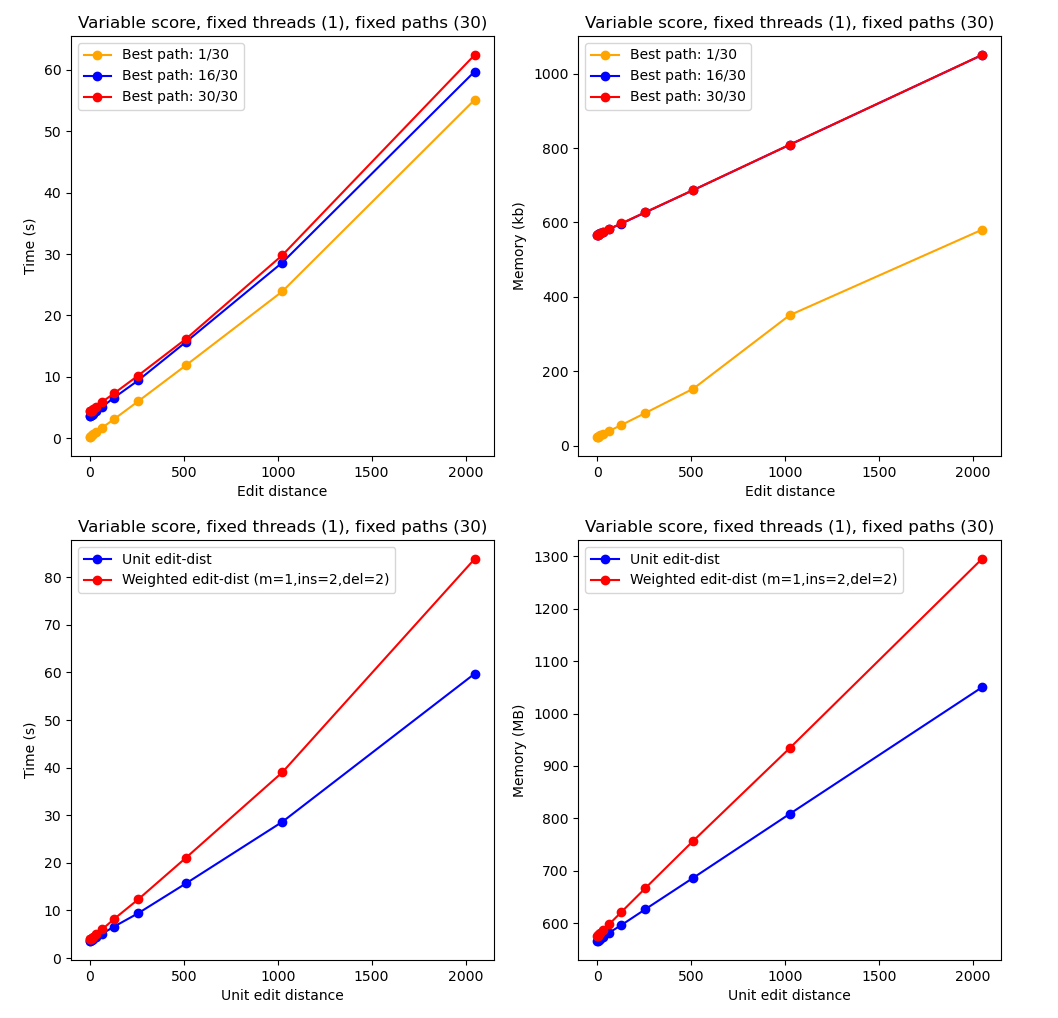
\includegraphics[width=1.0\linewidth]{images/benchmark_score_variable.png} 
        \caption[Andamento con score variabile]{Andamento in \emph{tempo} e in \emph{memoria} di \textbf{\textit{wf\_alignment}} rispetto a un \emph{punteggio} dell'allineamento \emph{variabile}.}
        \label{fig:benchmark_score}
    \end{figure}
    \vspace{20pt}
    
    Nella sperimentazione con \textbf{distanza di edit variabile} si nota un \emph{andamento lineare} sia in tempo che in memoria, in linea con le aspettative. Spostando la posizione del \emph{percorso ottimale} le rette mantengono lo stesso \textbf{coefficiente angolare}, variando nell'\textbf{ordinata all'origine} (conseguenza del troncamento rispetto alla soglia trovata, sezione \ref{section:wf_alignment}); aumentando le penalità, si nota un aumento dell'inclinazione della retta, conseguenza diretta della \emph{dipendenza lineare} nella \textbf{distanza di edit}.

\clearpage
\subsubsection{Numero di cammini del grafo variabile}
    \begin{figure}[h]
        \centering
        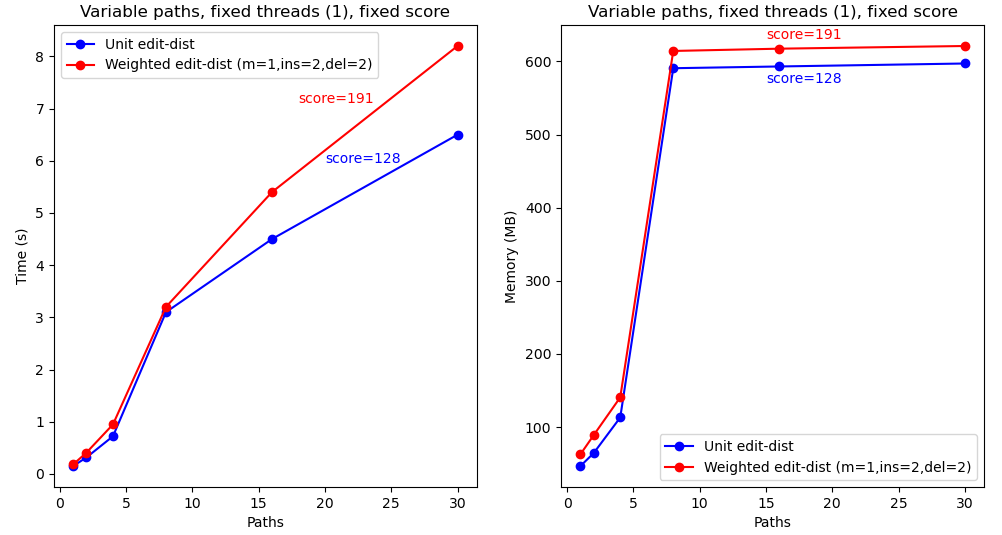
\includegraphics[width=1.0\linewidth]{images/benchmark_paths_variable.png} 
         \caption[Andamento con percorsi variabili]{Andamento in \emph{tempo} e in \emph{memoria} di \textbf{\textit{wf\_alignment}} rispetto a un \emph{numero di percorsi} del grafo \emph{variabili}.}
        \label{fig:benchmark_paths}
    \end{figure}
    \vspace{20pt}
    
    Nell'ultima sperimentazione, che considera il \textbf{numero di percorsi del grafo}, si ottengono risultati leggermente meno precisi dei precedenti, a causa dell'alta variabilità dell'input; infatti, il \emph{percorso ottimale} viene sempre inserito a metà dei percorsi disponibili: come conseguenza, i percorsi non ottimali (variabili) computati prima di quello ottimale provocano un andamento non completamente in linea con le equazioni \ref{equation:wf_time_complexity_benchmark} e \ref{equation:wf_space_complexity_benchmark}. Tuttavia, in assoluto è possibile comunque notare una \textbf{dipendenza lineare} nel \textbf{tempo di esecuzione}, mentre per quanto riguarda la \textbf{memoria} i risultati dipendono troppo dagli allineamenti trovati prima di quello ottimale.   


    \chapter{Conclusioni e sviluppi futuri}
    Il prototipo sviluppato dimostra a pieno le maggiori potenzialità dell'algoritmo \textbf{\textit{wavefront}} rispetto agli algoritmi di allineamento tradizionali, generando grandi risparmi sia in termini di \textbf{tempo} che in termini di \textbf{spazio} e permettendo di trattare istanze maggiori di diversi ordini di grandezza. Tuttavia, formalmente esso si basa sul calcolo della \textbf{distanza di edit} e non su un vero e proprio \textbf{allineamento}, producendo a volte risultati non in linea con quelli degli altri algoritmi; un importante futuro miglioramento è quindi sicuramente quello di estendere l'approccio \textbf{\textit{wavefront}} su \textbf{grafi di variazione} e \textbf{sequenze} per effettuare \emph{allineamenti con gap}\footnote{Una implementazione per i \textbf{grafi di sequenza} è già stata fornita nell'articolo \cite{wfa_gap_penalty}.}, che forniscono risultati più coerenti rispetto a quelli basati sulla \textbf{distanza di edit (pesata)}.   
    
    \vspace{10pt}
    Inoltre, nell'articolo \cite{wfa_sequence_graph} viene presentata un'\textbf{euristica} di \textbf{\textit{WFA}} che permette di ottenere ottimi risparmi di tempo, al costo di non avere la certezza di trovare la \emph{soluzione ottima}: l'\textbf{euristica} si integra molto bene con l'algoritmo, rendendo necessarie relativamente poche modifiche per implementarla all'interno del prototipo.
    
    \vspace{10pt}
    Infine, risulterebbe estremamente interessante riuscire a trovare un approccio che permetta di utilizzare l'algoritmo \textbf{\textit{wavefront}} su \textbf{grafi di variazione canonici} senza dover estrarre tutti i \textbf{percorsi} di quest'ultimi: un simile approccio permetterebbe di risparmiare grandi quantità di tempo dal calcolare più volte i valori per vertici appartenenti a diversi cammini (in maniera simile a quello che avviene in \textbf{\textit{RecGraph}}), rendendo tuttavia più complicato le computazioni in parallelo tramite \textbf{multithreading}.

    \vspace{10pt}
    In conclusione, l'\textbf{algoritmo \textit{wavefront}} rappresenta un'importante novità nell'ambito della \textbf{bionformatica}, che potrà portare a importanti miglioramenti in tutte le diverse applicazioni dell'\textbf{allineamento di sequenze}.  

    \bibliography{articles_stage, bwt}
    \bibliographystyle{abbrv} 

\backmatter
    %\input{chapters/6-postfazione}
    
\end{document}